% !TeX root = main.tex
\chapter{Paper-based semantic speech editing}\label{chp:paper}

In Chapter~\ref{chp:ethno}, we found that two of the three radio production teams we observed used paper as part of
their current production workflow.  We also saw that all of the radio producers we observed used transcripts to help
them navigate and structure their content.  In Chapter~\ref{chp:screen}, we saw that some radio producers found their
work environment noisy and distracting, and did not like working with screens for extended periods.  One of the study
participants chose to print their transcripts as they found the production process easier to achieve on paper than
directly on screen.

%A similar process happens in the production of media content. The production workflow typically involves recording
%material, selecting which parts of that material to use, then editing the desired material down to the final output
%\citep{Baume2015}.  Many producers will `log' the material after it is recorded by writing transcripts of what was
%said.  This is either done themselves or using a third-party service. These transcripts help producers to recall what
%was said and when, identify themes, and make links between different parts of their content.

Working on paper offers a number of advantages over working on screens.  Paper is lightweight, portable and does not
require any power, which allows users to work almost anywhere.  It is not back-lit, so is easier on the eyes.  It can
be navigated quickly, annotated freely whilst reading, and individual pages can be laid out and easily compared.  Its
physical low-tech nature also means that it is intuitive, robust, durable and does not crash or lose data.  Reading
from paper rather than a screen has been found to improve comprehension \citep{Mangen2013}, recollection
\citep{Singer2017}, sense of structure and cross-referencing \citep{OHara1997} and to be faster \citep{Kurniawan2001}.

Radio producers can use paper to make hand-written annotations to help them structure their program and make editorial
decisions.  However, printing a document breaks the link to its digital source, so is normally a one-way process in
which any information that is changed/added is not fed back.  For example, when a producer uses the paper transcript to
decide which parts of the audio they want to use in their programme, they must use a digital audio workstation (DAW) to
manually execute those editorial decisions, which is a tedious and slow process.  Creating a ``digital bridge'' between
paper and its digital source may allow us to combine the advantages of paper and digital workflows.

%Using this approach, it is possible to
%link the words on a printed transcript of speech to the time they were spoken in the original audio recording.
%Furthermore, by linking the paper annotations to audio edit commands, the paper transcript could be used to directly
%edit the audio content.

In this chapter, we describe the design, development and evaluation of \textit{Paper\-Clip} --- a novel system for editing
speech recordings directly on a printed transcript using a digital pen.  In Section~\ref{sec:paper-background} we
review previous approaches to semantic speech editing and natural annotation of digital content. In
Section~\ref{sec:paper-requirements} we describe our first study in which we worked with radio producers to design the
layout of our system. In Section~\ref{sec:paper-design} we describe the design of PaperClip, which we developed in
collaboration with a digital pen manufacturer. In Section~\ref{sec:paper-method} we explain the methodology of our
second study in which radio producers edited content for their programmes using PaperClip, a screen interface and a
normal printed transcript.  We present the results in Section~\ref{sec:paper-results} which compares the strengths of
the digital pen and screen interfaces, and shows how the accuracy of the transcript and listening affect the editing
process.  We discuss these results in Section~\ref{sec:paper-discussion} and present our conclusions in
Section~\ref{sec:paper-conclusion}.

%Transcripts are often printed out because:
%- it is easier to read than on screen
%- allows portability,
%- allows annotation,
%- flexible spatial layout
%- quick navigation
%- cross-referencing,
%- reduces battery anxiety,
%- more trusted by non-tech-savvy users

\section{Background}\label{sec:paper-background}

%Radio production using a paper interface requires a system that automatically translates annotations on a printed
%transcript to audio edit commands. Such a system requires a method of linking paper to media.  We identified three
%main approaches for achieving this, using barcodes, digital ink and digital pens.  In this section, we will review
%previous systems and studies that have used these techniques to link media with written documents.

Our system combines semantic editing of speech with natural annotation of digital content. As we saw in
Section~\ref{sec:background-semantic-editing}, previous semantic speech editing systems have all used screen
interfaces. We identified three alternative types of interfaces that could be used to edit digital content:
barcodes,
%\citep{Hull2003,Klemmer2003,Erol2007,Erol2008}
digital pens,
%\citep{Fouse2011,Guimbretiere2003,Conroy2004,Weibel2008}
and digital ink.
%\citep{Weher1994,Diakopoulos2006,Cattelan2008,Cabral2016}
In this section, we explore each of these approaches and their applications.

\subsection{Barcodes}
Barcodes printed on paper transcripts have been explored as a method of navigating video recordings by using a device
to scan the barcode and play the video from that position. \textit{Video Paper} \citep{Hull2003} was a system that
printed video keyframes and barcodes down the side of a paper transcript. Each barcode linked to a position in a video,
which was downloaded from a database and played on the scanning device. \textit{Books with Voices} \citep{Klemmer2003}
was a similar system that tested this approach on oral historians who found it effective for assisting a transcript
editing task. \citet{Erol2007} went a step further by embedding the video data in the barcode, removing
the need for a database.  \textit{HotPaper} \citep{Erol2008} removed the need for barcodes by using a camera to measure
the whitespace between words and matching that to unique patterns in the text.

Barcode-based systems provide a link between text and media. They use real paper, can be annotated freely, are easy to
generate and are robust to photocopying.  However, they do not provide a convenient method of capturing annotations. It
would be possible to use a handheld device to capture annotations and link them to a particular barcode.  However, this
would require the annotations to be entered into a handheld device, rather that just written on the paper.
Additionally, the size of barcodes means that they cannot be used for each word, which affects the precision of the
system.

\subsection{Digital pens}

A digital pen looks and functions as a normal pen, but includes an on-board infrared camera that tracks the position of
the pen while it writes on paper. Digital pens must be used in combination with paper that has a unique non-repeating
dot pattern printed onto it using a standard colour laser printer.  By reading this pattern, the pen can calculate
exactly where it is when touching the page. The pen records its position up to 100 times a second.  Depending on the
pen and software, this information can either be streamed live via Bluetooth, or downloaded as a batch onto a computer.
The digital pens that use this patented technology \citep{Fahraeus2003} are exclusively manufactured and licensed by
Anoto Group. As such, this technology is commonly referred to as the \textit{Anoto dot pattern}.

\textit{ChronoVis} \citep{Fouse2011} was a note-taking system that used the Anoto pattern for recording synchronised
hand-written notes during playback of a video. An accompanying screen interface allowed users to click on the digital
display of the handwritten notes to navigate to that position in the video. % or browse a list of timestamped notes.
\citet{Weibel2012} conducted a longitudinal study of ChronoViz for use in observational research. The results show that
notes became a mixture of linear notes and symbolic representations.  Asterisks, stars, lines and simple shapes were
used as bookmarks for later referral, or for counting events.  The flexibility of freehand notes also enabled use of
arrows in various contexts, such as to indicate direction and actions.

\textit{PADD} \citep{Guimbretiere2003} was a concept for a system of editing documents that used the Anoto pattern to
allow users to move from digital to paper and back again.  \textit{ProofRite} \citep{Conroy2004} was the first full
implementation of a PADD system, which overlaid annotations made on paper into a word processor. The annotations are 
anchored to the text, such that they ``reflow'' when the text is moved.  Through informal feedback, users suggested
that their annotations should translate into actions such as delete.  \textit{PaperProof} \citep{Weibel2008}
interpreted edit annotations and automatically applied them to the document.  Gestures for delete, insert, replace,
move and annotate were translated into modifications in a word processor, and intelligent character recognition was
used to digitise any hand-written text. The interpretation of annotations allows for a two-way interaction between the
digital and paper representations. We could not find any user studies of the PaperProof system.

%ChronoVis \citep{Fouse2011} used the Anoto dot pattern to record paper notes during playback of a video. After writing
%the notes, an on-screen playback interface allowed users to click on the digital display of the handwritten notes to
%navigate to that position in the video,
%Alternatively, they could reprint their
%notes and use a wirelessly-connected digital pen to tap on the notes, which controlled the playback position.
%ChronoVis can also coordinate multiple data sources, such as GPS logs.

%\citet{Conroy2004} created
%`ProofRite', which was the first full implementation of a PADD system. It captured annotations made to a printed text
%document, and overlaid the annotations onto the text in a word processor. The annotations were anchored to the text,
%such that they `reflow' when the text is moved.

%\citet{Weibel2012} conducted a longitudinal study of ChronoViz for use in observational research. They studied how
%three research groups used the technology over a period of 18 months by observing their use of ChronoVis, and
%conducting regular focus group and brainstorming discussions.  The study found that the introduction of the system
%changed the note-taking practices of the participants.  Paper-digital notes introduce time as an additional
%structuring factor, and the authors discuss the tension between the use of time and space. They point out that
%`deciding when time, space or both are important in a paper-digital form is complex'.  One benefit of a paper-digital
%interface is that when the digital pen fails, the paper still contains important information, however this is not true
%for time information.  Based on feedback from this study, ChronoVis was enhanced with features to control video
%playback, automatically recognise specific symbols and add notes on top of existing notes.

\subsection{Digital ink}
\textit{Digital ink} refers to technology that digitally captures and responds to the movements of a pen, such as a
stylus.  Typically, digital ink systems use a device with a backlit screen and a touch-sensitive interface like a
tablet PC.  Several systems have experimented with using a stylus with interactive sliders to provide advanced control
for navigating video content. Examples include \textit{LEAN} \citep{Ramos2003}, \textit{Zlider} \citep{Ramos2005} and
\textit{MobileZoomSlider/ScrollWheel} \citep{Huerst2008}. However, these systems are limited to the navigation of
content, without changing or labelling it.  As we will see in this section, digital ink interfaces can also be used to
annotate and edit media.

\textit{Marquee} \citep{Weher1994} synchronised handwritten notes with a live video recording by using a horizontal
line gesture to mark a timestamp.  \textit{Dynomite} \citep{Wilcox1997} synchronised handwritten notes to a live audio
recording, and allowed the user to categorise their annotations using keywords, and to highlight regions of audio using
a button.  In the evaluations of each of their systems, \citet{Weher1994} and \citet{Wilcox1997} both found that users
took fewer notes when using the digital ink system, and that they wanted to go back and use the audio/video to improve
the notes afterwards.

%`Marquee' \citep{Weher1994} was a digital ink system for supporting the task of logging during a live video recording.
%Users could make synchronised handwritten notes by drawing a horizontal line to mark a timestamp, then writing their
%notes below.  Additionally, they could create a list of keywords, and add them to their notes by pressing them at the
%right moment.  Marquee was evaluated for note-taking during meetings with three participants. The study found that
%users did not partake in discussions while logging, which may prevent such a system being used during an interview.
%The freehand nature of the notes meant that it could easily handle the different styles of each user.  Users reported
%that they didn't feel they had to make as many notes as they normally would, because they could later refer back to the
%video recording. The authors also noted that videos can be further annotated during replay, allowing for an iterative
%logging process.

%`Dynomite' \citep{Wilcox1997} was a virtual notebook that recorded audio synchronously with digital ink handwritten
%notes. The user's notes could be assigned to different `properties', either before or after they were written, to
%indicate an action point, for example, or a user-specified keyword.  Users could also highlight a portion of the audio
%by pressing a `mark' button or making a specific gesture.  This would highlight the audio for a specified time period,
%unless the `extend' or `end mark' buttons were pressed.  Any notes made during this period were displayed in bold and
%the highlighted segments were displayed using colours on a horizontal timeline. An evaluation of nine users found that
%users took fewer notes when using the audio highlighting, and that they wanted to go back and use the audio to improve
%the notes afterwards. Both of these findings mirror those from \citet{Weher1994}.

\textit{Videotater} \citep{Diakopoulos2006} was another digital ink interface for segmenting and annotating
pre-recorded video clips. A vertical line gesture on a video timeline split the video into a clip, which could be
labelled with handwritten notes.  \textit{WaCTool} \citep{Cattelan2008} also included features for annotation, but
added real-time collaboration and editing tools.  Users could assign a ``skip'' command, which is analogous to removal,
by pressing buttons at the start and end of an unwanted region.  \textit{Video as Ink} \citep{Cabral2016} allows users
to ``paint'' video frames onto the tablet interface and then edit the video by erasing unwanted frames.  Videotater,
WaCTool and Video as Ink all rely on the manipulation of video thumbnails, which are unavailable in radio production.

%\citet{Diakopoulos2006} developed a digital ink interface for creating and annotating segments of a pre-recorded video,
%called `VideoTater'. Segments could be created by drawing a vertical line on a video timeline, and merged by drawing a
%horizontal line between them. Each segment could be tagged by selecting it and hand-writing text. The back of
%the pen could be used to erase tags.

%\citet{Cattelan2008} added functionality for marking edit commands using digital ink in their system `WaCTool'.  Users
%could use a pen to write annotations by tapping the video to freeze it, then drawing on the video frame.  Users could
%apply a `skip' command to a segment of the video by using the pen to tap the bottom left of the video at the start of
%an unwanted segment, and tapping the bottom right at the end. The `skip' command is analogous to removing part of the
%video.  Similar commands for looping and slow motion were also available by tapping different regions.

%`Video as Ink' \citep{Cabral2016} took an alternative approach by allowing users to `paint' video frames and segments
%onto a 2D canvas using a pen and tablet interface. The canvas works as a timeline, but extends vertically in both
%directions so that the video can be painted onto multiple rows.  An evaluation of 12 participants found that the
%canvas allowed users to creatively explore different possibilities. However, the interface relies on the visual
%organisation of images, which does not necessarily translate well to audio and text.

Finally, as we saw in Section~\ref{sec:background-semantic-editing}, \textit{RichReview} \citep{Yoon2014} allowed users
to trim or tidy voice recordings by drawing a line through words or pauses to remove them.  An evaluation with 12
students found that the editing features were considered easy to use and efficient for removing ``umm''s and long
pauses.

\subsection{Summary}
In this section, we have seen that barcodes, digital pens and digital ink have been used to link paper to digital
media.  Barcodes are a simple way to achieve this using real paper, which can be annotated freely and is easier to
read.  Although an additional device is needed to capture annotations, a camera on a mobile phone could be used to read
the barcodes and play the digital content.  However, barcodes only provide a one-way link from paper to media as
annotations on the paper are not captured.  Barcodes also occupy space on the page, which limits the precision with
which they can be used.

Digital ink interfaces have both a screen and a stylus. This allows them to both capture freehand annotations, and
respond by replaying the original media, or erasing mistakes in the annotations.  However, as digital ink interfaces
use screens, they do not benefit from the improved reading speed, comprehension and cross-referencing of paper. They
are often bulky, have a short battery life, and in the event of battery or device failure, the transcript and
annotations are lost.  Electronic paper is a technology that attempts to emulate the benefits of reading from paper.
Although it has been commercially successful through its use in e-readers, studies have found that e-paper has a higher
reading time, worse comprehension and higher eye fatigue than reading from normal paper \citep{Jeong2012, Daniel2013}.
Additionally, we could not find any systems that provided the level of interaction that would be needed to mark-up a
transcript.

%TODO GAP IN LITERATURE
% - previous paper or pen-based systems have concentrated on navigation and annotation
% - some simple editing functionality was present in digital ink systems, but these didn't use transcripts
% - PaperProof allowed editing of text, but this didn't link to media
% - haven't considered audio, only audio-visual; not always translatable (e.g. video as ink)

%Video editing functionality was present in \textit{VideoTater} \citep{Diakopoulos2006}, \textit{WaCTools}
%\citep{Cattelan2008} and \textit{Video as Ink} \citep{Cabral2016}. However, all of these systems relied on the
%manipulation of video thumbnails, which cannot be translated to audio editing. None of them considered text or
%transcript-based editing.

Digital pen interfaces combine many of the benefits of both barcode and digital ink interfaces. They use physical
paper, which is better for reading, but also allow a two-way interaction by capturing freehand annotation. The
pen-based interface is natural and familiar, and because the annotations are made on the paper itself, information is
both accessible and backed-up in the event of device or battery failure. However, a colour laser printer must be used
with proprietary software to print the required dot pattern, and the printouts cannot be photocopied. There is no easy
way to undo or erase annotations, although this is an inherent problem with pens in general.  We have seen that digital
pen technology has successfully been applied to text editing \citep{Weibel2008} and media annotation \citep{Fouse2011},
but we could not find any previous literature which has combined these approaches to allow semantic editing of speech
content.

% Time dimension - time vs spatial representation

% Multiple iterations

%=====================================================================================================================

%`The Audio Notebook' \citep{Stifelman2001} was a system that used a physical pen and paper interface in combination
%with a device that recorded audio synchronously with the page and vertical location of the written notes.  The device
%could also replay the audio from a page and display which notes relate to the current playback position using an LED
%scrollbar display at the side of the page. Users could also use the scrollbar to control the position of the audio
%playback.  A longitudinal study of six participants over five months again found that users needed to take fewer notes,
%and made more notes during replay. Two of the participants were reporters who used the system while recording
%interviews. One reporter made minimal notes during the interview, but replayed the interview and made additional notes,
%including star symbols to indicate important moments. They also extracted quotes of interest by typing them into a
%computer. The other reporter was skeptical of the system, so made detailed notes so not to rely on the audio. However,
%they were later able to use the system to recall bits of the interview, which was many times faster than their existing
%technique of fully transcribing the audio recording.

%\subsection{Screen-based}
%Transcript-based interfaces have already successfully been applied to both audio and video editing. SCANMail
%\citep{Whittaker2002} demonstrated the advantages of navigating voicemail recordings using a transcript, but did not
%include editing capabilities.  The LIDS Editor \citep{Apperley2002}, and later TRAED \citep{Masoodian2006}, used
%automatically-generated transcripts to allow users to navigate and edit lecture recordings by removing and rearranging
%sentences and words. Even though automatically-generated transcripts are imperfect, Whittaker and Amento found they are
%sufficiently accurate to allow navigation and editing \citep{Whittaker2004}.  More recently, Rubin \citep{Rubin2013}
%created a system for using editable crowd-sourced transcripts to create audio stories.  Similar techniques have been
%applied to video editing. SILVER \citep{Casares2002} was a video editor that had an editable transcript window,
%generated from subtitles, and Berthouzoz et al.  \citep{Berthouzoz2012} developed a system that used crowd-sourced
%transcripts and image processing to allow text-based editing of multi-camera video interviews.

% Sensitivity of zones - a line which crosses from one zone to another can be a problem.
% Problems when line or symbols crosses over zone

%\subsection{Synchronised note-taking}
%A number of previous systems have explored how media can be annotated as it is recorded or replayed. These have often
%been developed for note-taking during meetings or lectures, but could also be applied to radio production. Although we
%did not find that it was commmon to write notes during interviews, we found that producers often listen back to their
%recordings, so these systems could be using during that replay process.

%\subsection{Correction}
%In chapter~\ref{chp:screen}, we identified that some producers were interested in correcting the transcript for sharing
%with others, or for later publication.

%TODO There are clearly defined symbols for use in proof correction (e.g. \citet{ISO5776}).

%TODO Interfaces to correct errors in transcripts have also been considered, such as that from \citet{Suhm2001}.

\section{System requirements}\label{sec:paper-requirements}

We developed a paper-based semantic speech editor for radio producers, to explore how it affects the production
process.  In this section, we describe how we evaluated a mock-up prototype to gather requirements for the design of
our system.

We chose to use digital pen technology because it uses paper, which provides better readability, and can capture
natural handwritten annotations.  Due to the lack of open development platforms, we collaborated with the digital pen
manufacturer Anoto to build our system.  We used their \textit{Live\texttrademark Forms} platform, which allowed us to
capture digital information from handwritten annotations.  The system worked by dividing a page into rectangular active
zones. When a compatible digital pen drew inside one of these zones, that data was captured digitally and processed.

In order to build our system, we needed to design the layout of the paper document and define a set of gestures for
editing the audio.  As there were no previous systems on which to base our design, this process raised a number of
questions about what information we should include in the layout, and which gestures we should use for interaction.
Specifically we were interested in answering the following questions:

  \begin{itemize}
    \item How do producers currently annotate transcripts?
    \item Do producers prefer to select or remove content?
    \item Which additional features (e.g.  timestamps, speaker labelling, confidence shading) should be included with
          the transcript?
  \end{itemize}

To answer these questions, we used paper prototyping to create a mock-up of our paper interface. For the mock-up, we
used a normal pen rather than a digital pen. This did not process the gestures, but otherwise provided an identical
experience.  This allowed us to test an initial design of our interface with users before building the functional
system.

%% Decided to use digital pens
%In the background, we saw that digital pens have successfully been applied individually to text editing and media
%annotation. We aimed to combine these into a paper-based audio editing system for radio production. We chose to base
%our semantic editing system on digital pen technology over digital ink and barcodes as it combines many of the benefits
%of each, is highly portable, and uses paper, which provides better readability and more natural interaction.

%% Collaborated with Anoto
%Digital pen technology is based on a set of techniques that are protected by a number of patents \citep{Fahraeus2003}.
%These are owned by Anoto Group, who exclusively license this technology and manufacture a number of products. Creating
%custom solutions can be expensive, so we collaborated with Anoto to develop our audio editing system.  Anoto gave us
%access to their Live Forms platform, which is designed for processing documents to capture digital information from
%handwritten annotations.

%In order to build our system, we needed to design the layout of the paper document and define a set of gestures for
%editing the content.  As there were no previous systems on which to base our design, this process raised a number of
%questions about what information we should include in the layout, and which gestures we should use for interaction.
%Specifically we were interested in answering the following questions:

%{\singlespacing
  %\begin{itemize}
    %\item What gestures are currently used by radio producers to annotate transcripts?
    %\item Do producers prefer to select content they want to keep, remove content they don't want, or a mixture of both?
    %\item Which additional features (e.g. timestamps, speaker labelling, confidence shading) should be included in the
      %layout?
  %\end{itemize}
%}

\subsection{Mock-up design}

In the results from Chapter~\ref{chp:screen}, we saw that radio producers annotated paper transcripts using underlining
(for selecting words), strikethrough (for removing words) and drawing a line down the side of the page (for selecting
whole lines).  We used this information as the basis for the design of our mock-up system, shown in
Figure~\ref{fig:paper-prototype-design}.

\begin{figure}[h]
  \centering
  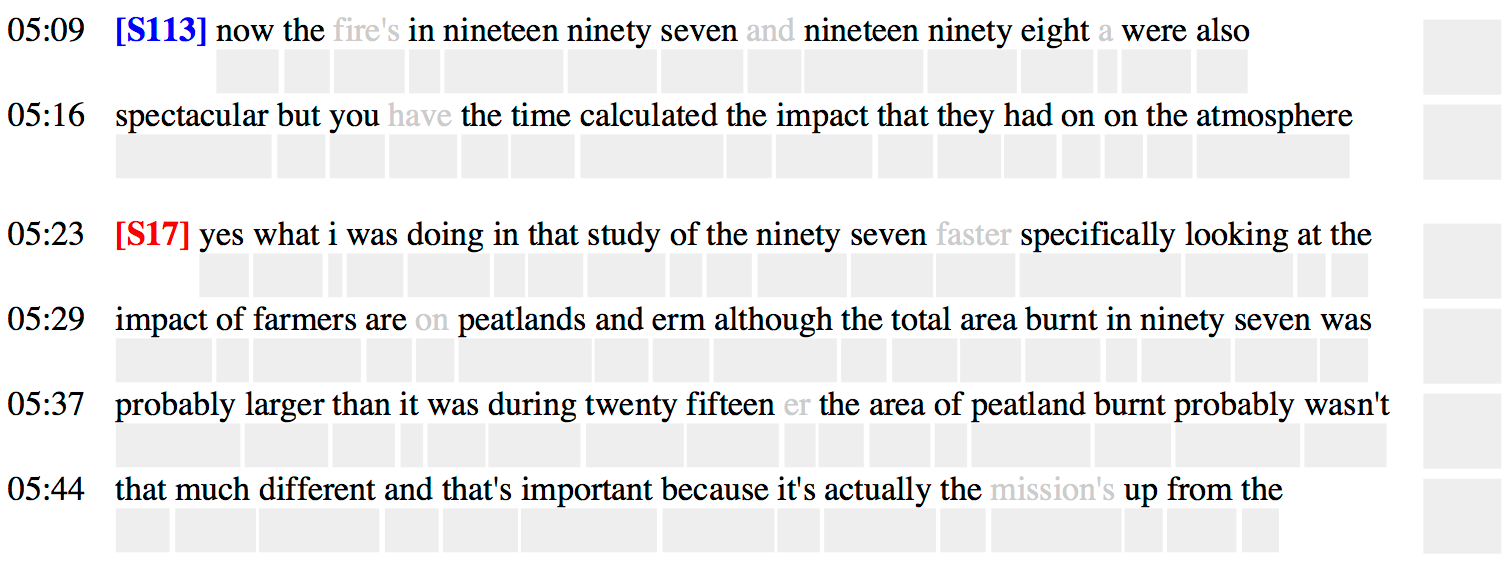
\includegraphics[width=\columnwidth]{figs/paper-prototype-design}
  \caption[Design of our paper mock-up.]{Design of our paper mock-up.  Words are selected by drawing in the box beneath
  the word, and removed by drawing over the word. A whole line is selected by drawing in the box to the right.
Timestamps are shown on the left.  Speaker turns are labelled with the speaker ID and coloured by gender. Words with a
low confidence score are shaded.}
  \label{fig:paper-prototype-design}
\end{figure}

We used an ASR transcript and included the additional information that was generated by the ASR system.  We wrote a
timestamp at the beginning of each line in \textit{minute:second} format, and used confidence shading \citep{Vemuri2004}
to ``low-light'' words with a low confidence score by shading them grey. We also put a paragraph break at speaker
boundaries and wrote the speaker label at the start of each paragraph. To distinguish speaker gender, we coloured the
speaker label blue for males and red for females.

To be able to capture timed edit commands using the \textit{Live\texttrademark Forms} system, we designed our layout to
use rectangular active zones that aligned with the location of each word.
%Traditionally this is used to detect when someone has ticked a box on a form, or to extract an image of a signature
%drawn inside of a box.  To capture edit annotations that linked to the text of the transcript, Edit commands: selector
%beneath word (double-spaced) and at end of line, removal by crossing word
We placed an invisible active zone over each word to capture strikethrough, a shaded active zone under each word to
capture underlining and a square shaded active zone at the end of each line to capture lines down the side.

\subsection{Mock-up evaluation method}

To evaluate our proposed layout, we recruited five radio producers (P1--P5) from BBC Radio to use our inactive
prototype to annotate real transcripts as if they were editing them.  Two of the participants worked in current
affairs, two in science and one in documentaries.  The participants had between 7 and 13 years experience in working as
radio producers.  Producers are very busy, so to recruit enough participants in the time available, we designed the
experiment to take less than one hour.  To make the study as realistic as possible, we asked each participant to
provide a recent interview recording they had made, which we used to generate an ASR transcript.

To help explore our questions about annotation and editing gestures, we directed participants to employ three different
strategies when using the prototype. This forced them to try different ways of interacting with the prototype, which
they could later reflect on and compare.  As part of the evaluation, we were interested in learning what gestures
producers currently use, or want to use, without being influenced by the design or constraints of the prototype.
We were also interested in directly comparing the underlining and strikethrough strategies.

We instructed the participants to follow the directions below for the first three pages of their transcript.

%TODO Explain interview protocol and analysis

%TODO Why are participants asked to adopt three different strategies?

%TODO Explain design decisions, e.g. double-spacing, confidence shading

\begin{itemize}
  \item Page 1: \textbf{Undirected} --- Edit the speech by annotating the transcript as you would normally.
  \item Page 2: \textbf{Underlining only} --- Edit the speech only by underlining words that you want to keep.
  \item Page 3: \textbf{Strikethrough only} --- Edit the speech only by putting a line through words you don't
        want to keep.
\end{itemize}

To evaluate speaker labelling, we excluded the labels from the first three pages, then included them on page 4
and asked the participant to edit the speech how they wished.  Timestamps, line selection and confidence shading were
included with all of the prototypes as we expected participants to be able to judge their value in situ.

After the editing task, we conducted a semi-structured interview with each participant.
%We categorised their responses into natural gestures, semantic gestures and additional features. 
We asked the following questions, but also allowed participants to talk freely.

{\singlespacing
  \begin{itemize}
    \item How do you normally use a pen to edit the transcript?
    \item Do you prefer to select parts you want to keep, or remove parts you don't want to keep?
    \item Which features of the prototype did you find useful?
    \item Were there any features missing that you would want added?
  \end{itemize}
}

We categorised their responses into natural gestures, edit gestures and additional features. We counted the frequency
of each response within the categories to compare the popularity of the features and editing strategies.

%We were also interested in learning about additional features and their value. To get feedback on the value of speaker
%diarization, we produced two versions of each participant's transcript --- one with speaker diarization and one without.
%The speaker information was used to segment the transcript into paragraphs, and the start of each paragraph was
%labelled with the speaker identifier in square brackets (e.g.  \texttt{{[}S1{]}}).  For \textit{Page 4}, each
%participant was presented with a transcript that included speaker diarization, and asked to edit the speech by
%annotating the transcript any way they wished.

%Timestamps, line selection and confidence shading were included with all of the prototypes. For these features, we
%chose not to produce versions with/without to reduce the number of permutations. We expected that participants should
%be able to judge their value without having to see them removed, and producing different versions for each would have
%unduly lengthened the experiment.

\subsection{Mock-up evaluation results}

The reaction to the system was overwhelmingly positive. All of the participants could immediately see the value of such
a system and most remarked that it would save them significant amounts of time.

Table~\ref{tab:natural-gestures} lists the gestures that the participants used when editing undirected on pages 1 and
4.  Each participant naturally used a different mixture of gestures for selection, removal, correction and labelling.
The most common gestures for selection were underlining and line down side, with strikethrough being the most common
removal gesture.  Most participants combined line down side for large selections with underlining and strikethrough for
finer edits.

\begin{table}[h]
  \centering
  \begin{tabular}{l c c c c c c}
    \hline
    & \textbf{P1} & \textbf{P2} & \textbf{P3} & \textbf{P4} & \textbf{P5} & \textbf{Count} \\
    \hline
    Underlining               & $\bullet$ & $\bullet$ & $\bullet$ & $\bullet$ &           & 4 \\
    %\hline
    Strikethrough           & $\bullet$ & $\bullet$ &           & $\bullet$ & $\bullet$ & 4 \\
    %\hline
    Line down side          & $\bullet$ & $\bullet$ & $\bullet$ &           & $\bullet$ & 4 \\
    %\hline
    Comments                & $\bullet$ & $\bullet$ &           &           & $\bullet$ & 3 \\
    %\hline
    Corrections             & $\bullet$ &           &           &           & $\bullet$ & 2 \\
    %\hline
    In/out marks            & $\bullet$ &           &           & $\bullet$ &           & 2 \\
    %\hline
    Scribble-out mistake    &           & $\bullet$ & $\bullet$ &           &           & 2 \\
    %\hline
    Lasso                   &           &           &           &           & $\bullet$ & 1 \\
    %\hline
    Line through paragraph  &           &           &           &           & $\bullet$ & 1 \\
    \hline
  \end{tabular}
  \caption{Natural gestures used by each participant to edit their transcripts.}
  \label{tab:natural-gestures}
\end{table}

We asked each participant whether they preferred selecting or removing words when editing the transcript.  P1, P3 and
P4 reported that they preferred selecting, with P2 and P5 preferring to remove words.  P1 commented that selecting
\textit{``felt more natural''} to them, and P4 said deleting felt \textit{``counter-intuitive''}.  P2 and P5
reported that they preferred deleting words. P2 commented that \textit{``the challenge is to nibble away''} and it was
\textit{``the way my brain works''}.  P5 said they prefer to \textit{``get stuff out of the way''}.  All of the
participants were certain about which they preferred, but there was no overall consensus. Additionally,
Table~\ref{tab:natural-gestures} shows that most participants used a mixture of select and delete gestures during the
undirected stage.

Four of the five participants said that they found the paragraphs and speaker information useful. Typically, interviews
are recorded with a presenter and contributor, and the participants said they found it valuable to know when the
presenter is asking a question. Three of the participants said that they were able to find the questions much more
easily with this feature enabled. However, P2 said they found the speaker diarization to be \textit{``distracting''},
particularly when it was inaccurate.

All participants said they found the timestamps and confidence shading features useful, but P2 said that the timestamps
are \textit{``not needed on every line''} and P5 suggested that one timestamp per page would be sufficient.

All of the participants liked being able to select whole lines at a time. P5, who prefers to remove words, asked
whether a similar function could be available to delete content.

During our testing, some participants suggested adding features that were not included, or used the prototype in a way
it was not designed.  P3, P4 and P5 remarked that they often highlight important bits of transcripts, usually with
asterisks or stars.  P1 and P3 also suggested extending the underlining gesture so that underlining twice marked words as
being more important.  Three participants used what little space there was at the side to label the content and make
notes for themselves, and P1 and P5 corrected mistakes in the transcript by writing over or above the incorrect word.

%\begin{figure}[h]
  %\centering
  %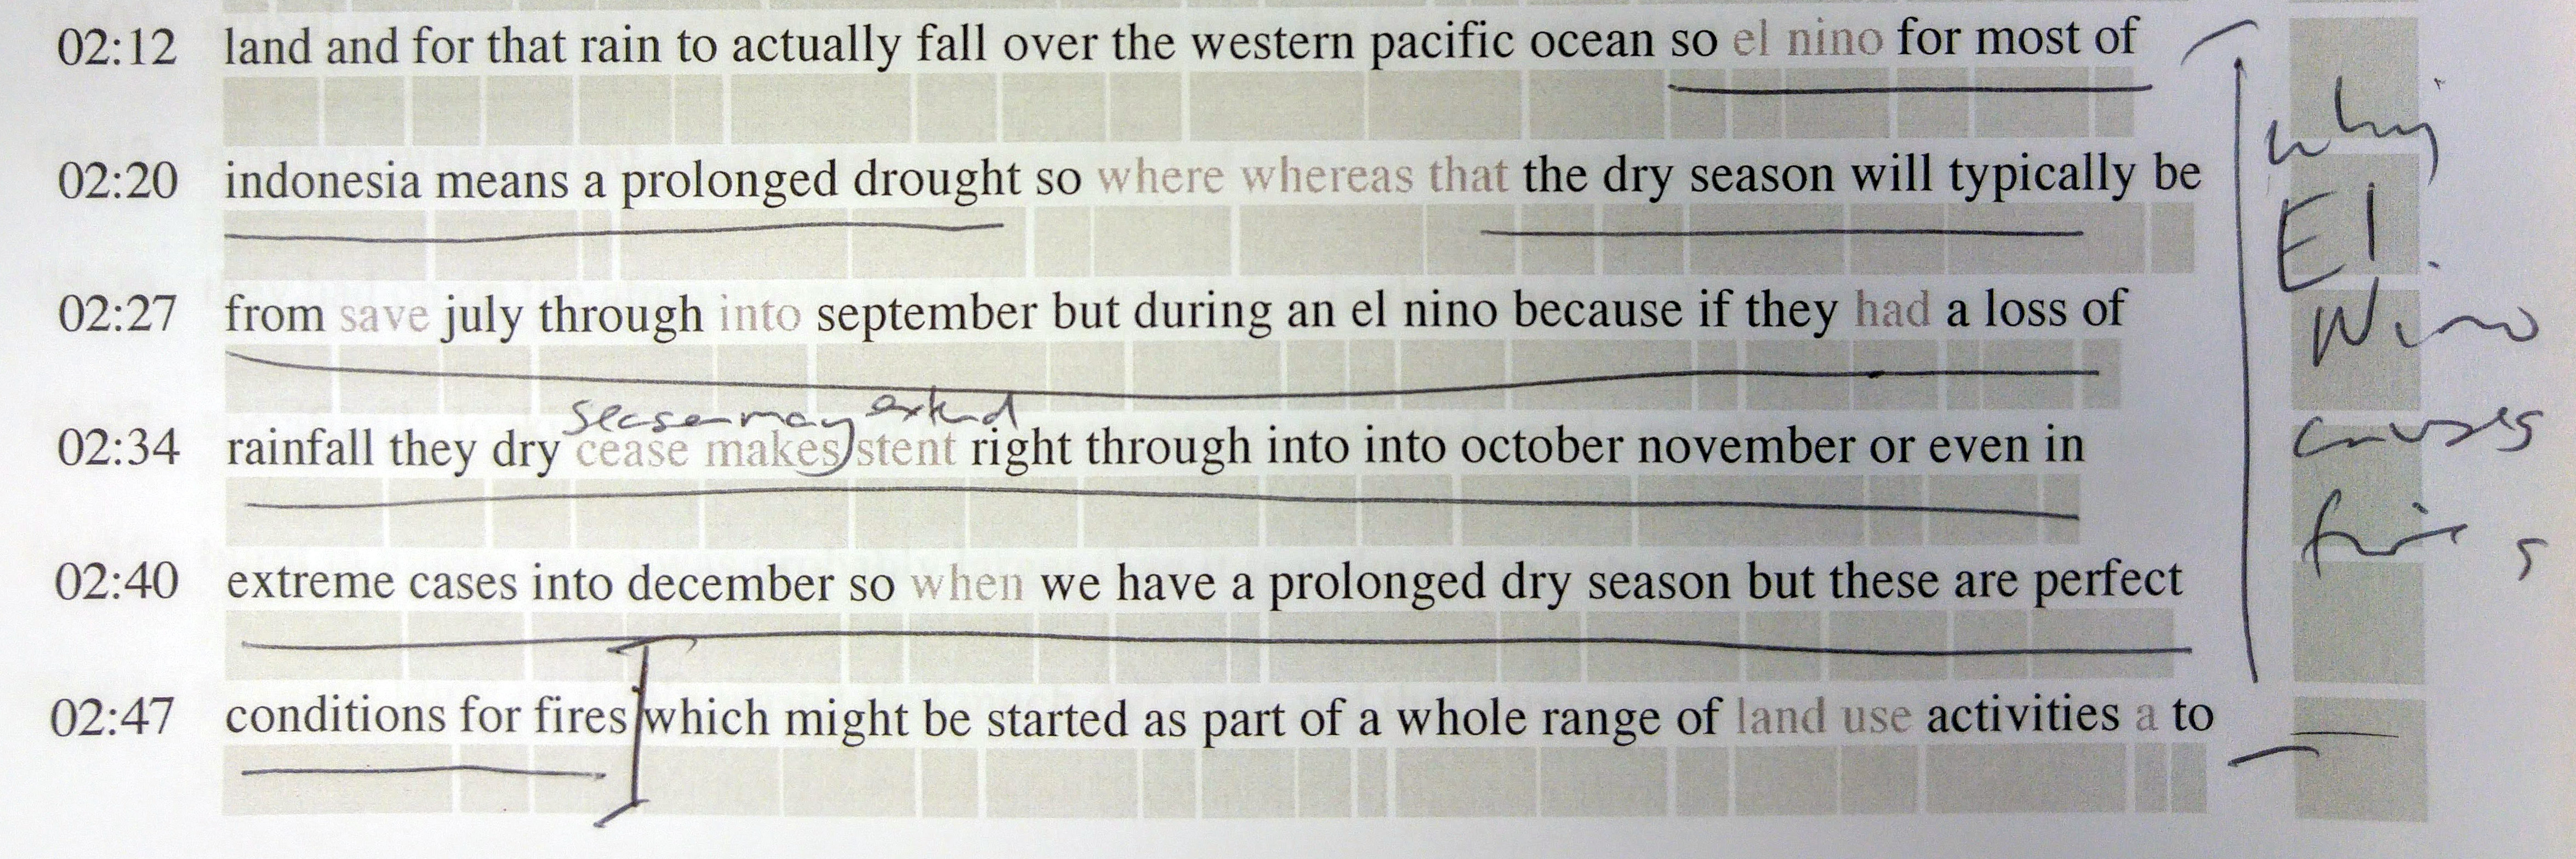
\includegraphics[width=\columnwidth]{figs/mockup-cropped}
  %\caption{Paper prototype with natural annotations, including
    %underlining, line down the side with notes, word corrections, and a
  %vertical line to indicate the end of an edit.}
  %\label{fig:natural}
%\end{figure}

%Four different gestures were used to select content --- underline, line down side, in/out marks and lasso.  Underline
%was used by all participants except for P5, who said they were mainly interested in deleted unwanted content.  Drawing
%a line down the side was used by three participants, as it is quicker and more efficient than underlining for selecting
%large chunks of material.  Some participants combined both by using underline to be more precise about the start and
%end of their selection.  One of the participants made a mistake when underlining, so scribbled out the underline to
%undo it.

%`In/out marks' refers to drawing short vertical or diagonal lines before and after the words of a selection. These
%indicate the in- and out-points for edits. One participant drew an analogy between these marks and the splicing of
%magnetic tape, which was how radio programmes were edited before the digital age. `Lasso' refers to selecting a number
%of words by drawing a line around them.

%Two gestures were used to delete content --- strikethrough and drawing a line through a paragraph. These are the
%opposite to the underline and line down side gestures that are used for selection, but instead involve drawing a line
%through the words themselves.
%%TODO Expand

%Finally, P1 and P5 corrected mistakes in the transcript by writing the correction over/above the
%word, or to the side of the page.
%%TODO Expand

%Each participant used a different mixture of annotation techniques.
%%TODO Expand

%\subsubsection{Edit gestures}\label{sec:paper-proto-edit-gestures}
%We asked each participant whether they preferred selecting or deleting words for editing the transcript.  P1, P3 and P4
%reported that they preferred selecting, P1 commented that it \textit{``felt more natural''} to them and P4 said
%deleting felt \textit{``counter-intuitive''}.

%P2 and P5 reported that they preferred deleting words. P2 commented that \textit{``the challenge is to nibble away''}
%and it was \textit{``the way my brain works''}. P5 said they prefer to \textit{``get stuff out of the way''}.

%All of the participants were certain about which they preferred, but there was no overall consensus. Additionally, we
%can see in Table~\ref{tab:natural-gestures} that all participants used a mixture of select and delete gestures during
%the undirected annotation.

%\subsubsection{Additional features}

%% speaker diarization
%Four of the five participants said that they found the paragraphs and speaker information useful. Typically, interviews
%are recorded with a presenter and contributor, and the participants said they found it valuable to know when the
%presenter is asking a question. Three of the participants said that they were able to find the questions much more
%easily with this feature enabled. However, P2 said they found the speaker diarization to be \textit{``distracting''},
%particularly when it was inaccurate.

%% timestamps/confidence shading
%All participants found the timestamps and confidence shading features useful, but P2 said that the timestamps are
%\textit{``not needed on every line''} and P5 suggested that one timestamp per page would be sufficient. All of the
%participants liked being able to select whole lines at a time. P5, who prefers to remove words, asked whether a similar
%function could be available to delete content.

%\subsubsection{Missing features}

%During our testing, some participants suggested adding features that were not included, or used the prototype in a
%way it was not designed.
%% highlighting
%P3, P4 and P5 remarked that they often highlight important bits of transcripts, usually with asterisks or stars.
%P1 and P3 also suggested that the underline gesture could be extended so that underlining words twice marks them as
%being more important.

%% labelling, margins
%Three participants made notes on the side of the page to label their content or to make a note for themselves. As there
%was no margin, the notes were often scrawled sideways in small writing. If the prototype was active, writing notes
%on the transcript itself would likely have triggered the active zones located on and below each word. This would cause
%the user to inadvertantly create edits to the audio. P3 suggested that it may be worth adding a margin. Providing an
%inactive margin would give users a `safe space' to make freehand notes without editing the audio.

%% correction
%Two participants corrected words in the transcript by writing over or above the incorrect word. As the transcript was
%double-spaced, there was just enough room between lines to write the correct word in small writing.
%% listening/playback
%P3, P4 and P5 expressed a desire to listen to the audio while reading/editing it, which echoes the importance of
%listening noted in Chapter~\ref{chp:screen}.

%- Useful to know where presenter is asking question

%Diarization
%- Neal found it easier
%- Shows where the questions are
%- Phil found it distracting
%- Wes found it absolutely useful
%- Marnie 'made it much easier', liked having paragraphs (usually one point per
%paragraph)


%Timestamps
%needed every couple of minutes

%Use L/R channels for presenter/contributor
%- Phil and Wes
%- Sometimes multiple on R channel (about one in eight interviews)

%Prefer landscape to portrait (landscape is `irritating' and doesn't match
%what's on screen)

%Whole line
%- Would like to delete line at a time

%Note-taking
%- One doesn't take many notes

%Correction
%- One corrects then selects edits
%- Wes would like option

%Highlighting
%- Asterix/star to mark important bits (Phil, Neal)
%- Underline twice (Neal, Marnie liked idea)
%- Wes sometimes double-stars

%Delete vs select (2 vs 3)
%- Phil likes to `get stuff out of the way'
%- Words that aren't marked should be kept by default
%- Underline should undo delete
%- Neal prefers selecting over deleting
%- Delete should undo select, if underlined too far
%- Wes prefers selecting - deleting is `counter-intuitive'
%- Would like delete to override select, but would like options for opposite
%- Marnie found it trickier to delete than select, selection is more natural
%- worried about deleting something good
%- Alex feels delete is more natural, 'way may brain works, 'challenge is to
%nibble away', thinks delete should be active, select should override delete

%Margin
%- Phil wouldn't need a margin
%- Neal would like one

%Export
%- gaps should be put between edits (real-time?)

%Transcript
%- Phil and Neal no problems
%- Wes had problems (strong Scottish accent) made it unusable

%Observation
%- Neal
%- underlined as he read (unprompted), scribbled out when mistake made
%- found it more difficult to only delete
%- Wes
%- vertical lines for in/out points

%Other
%- Neal would like to press and hear word (on laptop?)
%- Wes: Don't know what sounds good
%- Wes works in a team of 3/4. They use Box to collaborate
%P4 reported that they usually work in teams of 3 or 4 people. They use Google Docs to collaborate on a central
%programme script, so they can all edit the document simultaneously.

\subsection{Requirements}

The results of our mock-up evaluation showed how radio producers currently annotate transcripts, that there are mixed
opinions on whether to select or remove content, and that they valued the additional features tested.  We also
discovered additional requirements for margins and highlighting that were not initially identified.  We will now use
these results to produce a set of design requirements for our system.

\paragraph{Edit gestures}
The most common edit gestures used by participants were underlining, strikethrough and line down side, with the other
gestures being used less than half as often.  This confirms our initial assumptions, so our design should use these
gestures for editing operations.

\paragraph{Select vs remove}
There were mixed but strong opinions on whether participants preferred to select or remove content, and most used a
mixture of both.  This indicates that both selection and removal should be made available. In cases where both are
used, remove should override select as this would allow users to draw a line down the side to select large chunks and 
to cross-out individual words within those.

%There is likely to be
%more interest in removing individual words, such as for removing ``umm''s, than there is for selecting individual words. For
%this style of use, it may be better for delete to override select.
%There were mixed but strong opinions on whether it was better to select good content or remove bad content.  Most
%participants used a mixture of both approaches when undirected.
%Given the lack of consensus, it would be best to give
%producers the option to do both, but this raises the issue of what should happen when a word is both selected and
%deleted.  If one overrides the other, then it could function as an undo mechanism. The more conservative approach would
%be for selection to override deletion, so that speech can always be recovered. However the system does not actually
%delete any audio, so this is not a risk.
%Selection and deletion could be used together at different scales, where one is used to select/delete large chunks,
%then the other is used to refine the choice by selecting/deleting smaller words or chunks within the larger ones.
%In our results, we saw that selecting large chunks is more popular than deleting large chunks. Also, there is

\paragraph{Additional features}
Most participants valued speaker diarization, timestamps and confidence shading, so these additional features should be
included.  However, some participants reported that timestamps on every line are unnecessarily frequent and that one
per page would suffice.

\paragraph{Margin}
Three participants made notes on the side of the page to label their content or to make a note for themselves, and two
suggested adding a margin. With the \textit{Live\texttrademark Forms} system, writing notes on the transcript itself would trigger the active
zones that are on and below each word. Our design should include an inactive margin, as this would allow users to make
freehand notes without inadvertently making edits to the speech.

\paragraph{Highlighting}
The ability to highlight regions of interest was a desired feature. Two participants suggested double underlining could
be used to achieve this, however, this may be hard to detect using the \textit{Live\texttrademark Forms} system.
Alternatively, by giving the user an option to keep all of the content except for deleted words, underlining could then
be used to highlight parts of interest. This mode-switching design would give the user greater flexibility in how they
use the system.

% highlighting
%Most participants remarked that they normally mark important bits of the transcript, often with asterisks or
%stars. Underlining twice could also introduce a two-tier selection system.
%Possibly the side boxes could be used to rate or star a selection.

%==================================================

%In this section, we set out to answer three questions about the gestures producers use to edit printed transcripts, and
%which features we should include in our paper-based audio editing interface. We did this by evaluating a paper
%prototype of our interface on five radio producers using real content.

%\item What gestures are currently used by radio producers to annotate transcripts?
%\item Do producers prefer to select content they want to keep, remove content they don't want, or a mixture of the
%two?
%\item Which additional features (e.g. timestamps, speaker labelling, confidence shading) should be included in the
%layout?

%We observed that the participants used a variety of gestures to select and delete content, with underline,
%strikethrough and a line down the side being the most common.  This confirms our assumptions about these being the most
%popular annotations. The other gestures included in/out marks and lasso for selection, and drawing a line through a
%paragraph for deletion.  In \citet{Weibel2008}, strikethrough was also used for delete, but something similar to in/out
%marks was used for annotating a specific region.



% Missing features
%Handwritten text was also used to make
%corrections to the transcript, and to label parts of the transcript.


% playback
%Some participants expressed a desire to listen to the media from the paper interface, such as was possible in
%\citet{Fouse2011}.  An external device, such as a phone, computer or portable media player could be used to replay the
%audio while using the paper interface.  Users could start playback by pressing a word with the digital pen. This could
%be achieved either by wirelessly linking the digital pen to a computer that plays the content, or by storing the audio
%on the pen itself similarly to the LiveScribe Sound
%Stickers\footnote{\url{http://store.livescribe.com/sound-stickers-1-1.html}}.

% natural annotation:
% underline, strike and line down side most used, reinforced design decision
% comments and correction were popular, no space to write them
% in/out marks, lasso also used for selection, line through paragraph used for deletion, but to lesser extent

% edit gestures:
% no consensus on best approach, both used when naturally annotating, so both should be available
% what to do when using both? underline override strike or vice-versa?

% additional features:
% speaker diarization - yes
% timestamps - yes, but less frequently
% confidence shading - yes


%Our system performs the same function as these systems, but uses a paper
%interface rather than a screen-based one.
%Our system
%similarly interprets the paper annotations and applies them to the media
%content.
%Our system does not yet have the ability to replay content from the
%paper interface, but this is a feature that could later be included.
%Our system is based on printed transcripts rather than video frames on
%a tablet, but approaches the same problems from a different angle.
%These systems do not provide the user with any pre-written notes.
%Our system uses speech-to-text to generate a transcript, which the user can
%then annotate further.

%The participants used a variety of techniques to annotate the transcripts, but underline, strikethrough and lines down
%the side were common. There were strong but mixed opinions on whether selection of desired material, or removal of
%unwanted material, was the best approach to use for editing, so we decided to make both options available.

%TODO What happens when underline and strike same word?

\section{System design}\label{sec:paper-design}

%TODO Why are some desired features not included, e.g. vertical lines for in/out, lasso

%TODO How are the results of the edit presented back to the user?

%TODO Underline/strikethrough interaction


Using the requirements gathered from our mock-up evaluation, we designed and implemented a working prototype of the
paper-based semantic speech editing system.  Previous semantic speech editing systems have used screen interfaces. In
order to have a baseline by which to compare the effect of paper-based semantic editing on radio production, we also
implemented a screen interface. This section describes the design and implementation of both of these systems.

\subsection{Paper interface}

Based on our findings, we used underlining, strikethrough and line down side as the edit gestures, and included speaker
labelling and confidence shading.  We retained the timestamps, but reduced their frequency to one per paragraph, rather
than on every line.  We added an inactive margin to allow users to write freehand notes without the risk of
accidentally editing the audio.  We did this by drawing a rectangular box on the right side to indicate where the user
could safely write.  We set the width of the margin to be approximately 25\% of the width of the page, based on
informal feedback from producers.  Due to the wide variety of annotations that producers use, we did not attempt to
capture structured notes.

We collaborated with Anoto to implement PaperClip using their \textit{Live\texttrademark Forms} platform. As this
platform did not allow us to combine underlining and strike\-through gestures with handwriting recognition, we could
not include correction functionality.  We did not include integrated playback control, as this would require a wireless
link to the digital pen, which the platform did not support.

We used two active zones for each word --- one \textit{on} the word to detect a strikethrough, and one \textit{below}
the word to detect underlining. Drawing inside a zone would mark that word as either removed or selected, respectively.
We lightly shaded the zone below each word to make the boundary visible.
%We shaded the zone below so the user can see where the boundary lies.
We drew a long thin rectangle between the transcript and the margin for capturing a line down the side. The final
design is shown in Figures~\ref{fig:paper-interface-diagram} and \ref{fig:paper-interface-example}.

\begin{figure}[t]
  \centering
  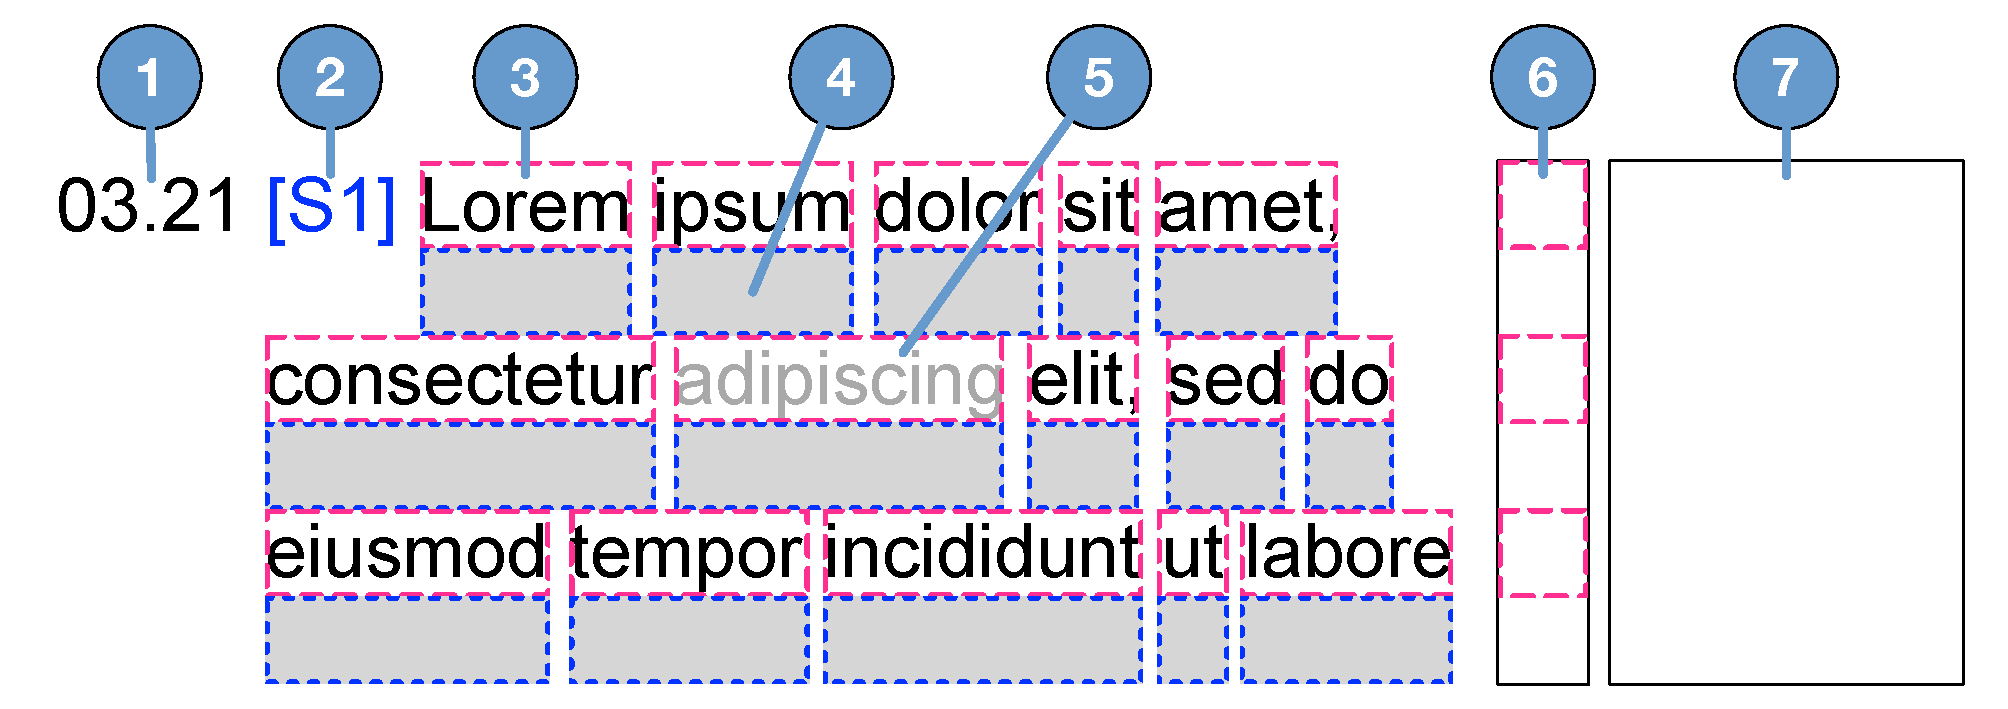
\includegraphics[width=\columnwidth]{figs/paper-interface-diagram.pdf}
  \caption[Layout of the paper interface.]{Layout of the paper interface, with timestamps at beginning of each
  paragraph (1), speaker diarization (2), word deletion (3), word selection (4), confidence shading (5), line selection
(6) and a margin for freehand notes (7). Dotted lines indicate hidden active zones for selection (pink) and deletion
(blue).}
  \label{fig:paper-interface-diagram}
\end{figure}

\begin{figure}[p]
  \centering
  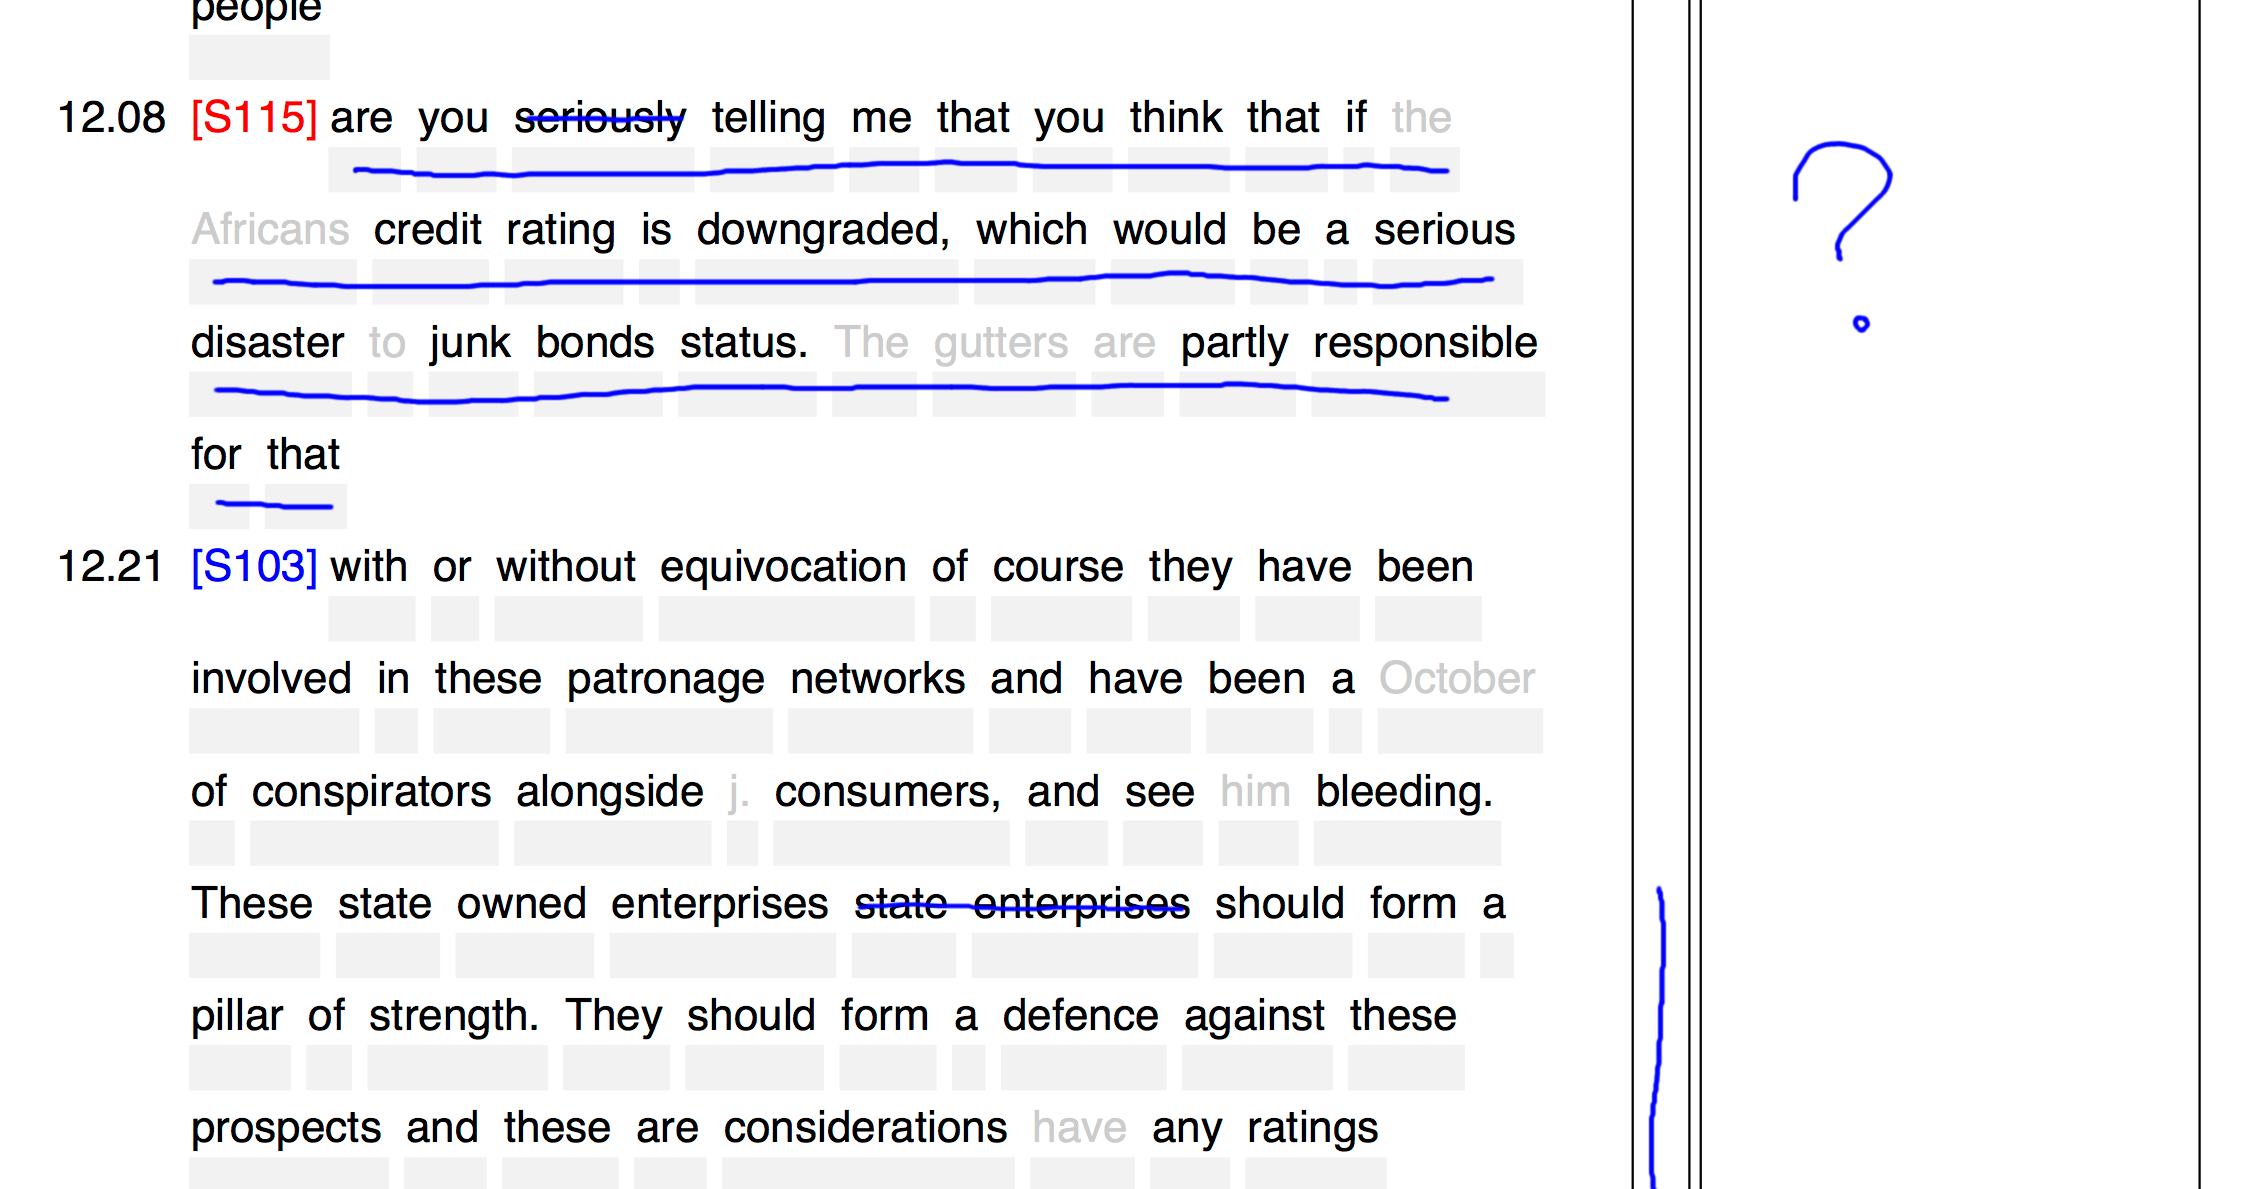
\includegraphics[width=\columnwidth]{figs/paper-interface-example-annotations.png}
  \caption{Example of the paper interface system, with freehand annotations that demonstrate its use.}
  \label{fig:paper-interface-example}
\end{figure}

\begin{figure}[p]
  \centering
  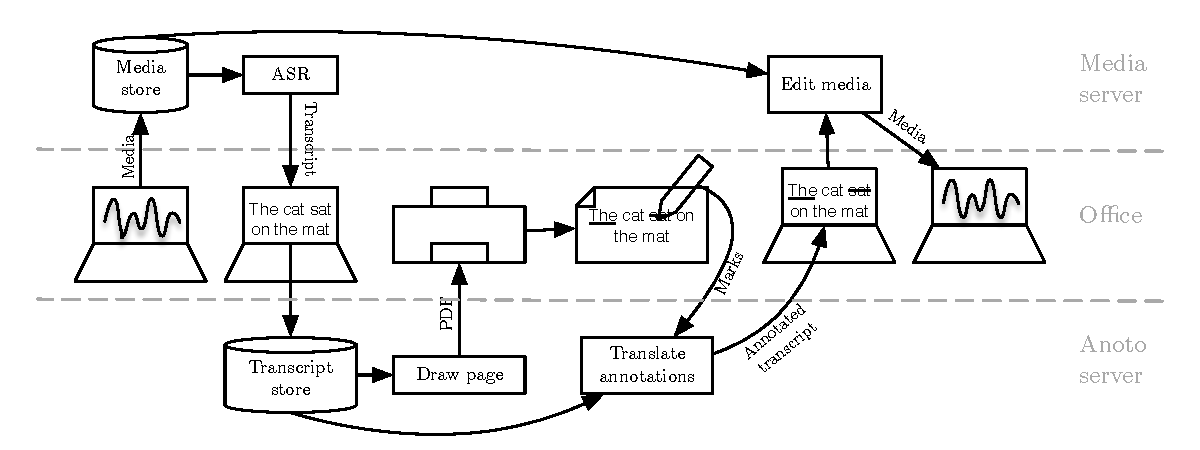
\includegraphics[width=\columnwidth]{figs/uist-sys-diagram}
  \caption{Flow diagram of PaperClip, showing the integration between the paper and screen interfaces, flowing from
  left to right.}
  \label{fig:paper-screen-integration}
\end{figure}


Editing was performed using an Anoto Live Pen 2 digital pen, which tracked and digitally recorded the gestures made on
the transcript.  When the pen was connected to a computer via a USB dock, the gestures were processed and translated by
the Anoto system into edit commands.  We integrated PaperClip with our screen interface (see
Section~\ref{sec:paper-screen-design}) to handle audio import, printing transcripts, viewing/changing edits, viewing
the margin notes and exporting the edits.  A diagram of this integration is shown in
Figure~\ref{fig:paper-screen-integration}.

We supported two export formats --- audio as a WAVE file, or an edit decision list (EDL) for the SADiE or StarTrack
DAWs.  PaperClip also created a PDF document of the transcript that showed the user's annotations, which could be
viewed through the screen interface.

%\subsubsection{Design decisions}

%We chose to use three methods for selecting and deleting material - underline, strikethrough and line down the side.
%We did not include in/out marks, lasso or drawing a line through a paragraph as these were not as popular, and would
%have been difficult to detect using the Anoto Live Forms system.

%We included speaker diarization and confidence shading, as the majority of participants in the paper prototype found
%these valuable. We also chose to keep timestamps, but opted to reduce the frequency to one timestamp per paragraph,
%rather than on every line. We expected this to provide a sufficiently narrow search area without cluttering the page.

%We added an inactive margin to allow users to write freehand notes without the risk of accidentally editing the audio.
%We did this by drawing a rectangular box on the right side to indicate where the user could safely write.  We set the
%margin to be approximately 25\% of the width of the page, based on informal feedback from producers.  For the margin,
%we decided to allow users to draw freehand in the margin, rather than attempt to structure and capture these
%annotation. We did this because there were a wide variety of annotations and techniques that producers use for
%annotations.

%In the paper prototyping experiment, we saw that some participants wrote corrections on or above wrongly transcribed
%words. However, we chose not to include any correction functionality, partly due to the limitations of the Live Forms
%system, and partly to keep the interface simple. The active zones on or below each word could have been used to write
%corrections, but this would prevent underline or strikethrough gestures being used. The correct word would also have to
%be written within these active zones, which are quite small. Some corrections span more than one word, which would be
%difficult to detect.

%We did not include any linked playback features as this would require a live wireless link between the pen and a
%playback device. We only had access to the Anoto Live Forms system that operated in batch mode, where the pen must be
%connected to a dock to upload the recorded gestures. Although this prevented the user from navigating the audio using
%the pen, they could still replay the audio on a separate device and use the timestamps to navigate to the correct
%location.

%\subsubsection{System description}

%This section describes the final design we used for the paper interface for our semantic speech editing system.
%Figures~\ref{fig:paper-interface-diagram} and \ref{fig:paper-interface-example} on page
%\pageref{fig:paper-interface-diagram} show the final design of the interface.

%For each word in the transcript, two rectangular active zones are defined on the page --- one on the word itself and
%another in the space directly below the word.  Any marks made on or below the word label that word as `deleted' or
%`selected', respectively.  This allows the user to use a digital pen to mark words as deleted using a strikethrough, or
%to mark words as selected by underlining.  The zone below is lightly shaded so that the user can see where the boundary
%lies between the two regions.

%For selection by drawing a line down the side, we opted to draw a long thin rectangle from the top to the bottom of the
%page to the right of the transcript, rather than draw individual square boxes at the end of each line. We did this to
%save some space, and to align with how the participants used the paper prototype.

%To include audio editing functionality with the pen system, we integrated it with a screen-based interface. A diagram
%of this integration is shown in Figure~\ref{fig:paper-screen-integration}. The screen was used for asset management,
%including uploading new content, printing the transcript, viewing/changing the edits made using the pen, and exporting
%the resulting audio or edit decision list.

%The paper must be annotated using an Anoto Live Pen 2. This records the gestures made by the users digitally on the
%pen.  When the pen is connected to its USB dock, the gestures are automatically uploaded to Anoto's software running
%on the local computer, which processes the information from the pen. This is then sent to our server, which creates an
%edited version of the transcript. This can then be accessed through the screen interface.

%In addition to creating an edited version of the transcript, a PDF document of the transcript with the user's
%annotations is created. This PDF can be viewed through the screen-based interface, so that they can view any notes
%they made in the margins.

%The user can export the audio from the edited transcript using the screen interface. Two types of export format are
%supported. The user can download an EDL of the edits for either the SADiE or StarTrack audio editing systems.
%Alternatively, they can download an edited version of the audio as a WAV file.

%Anoto wrote the software that draws the transcript onto the page, and the software that translates the pen annotations
%into structured data. These can be seen on the left side of the diagram in Figure~\ref{fig:paper-screen-integration}.
%We built the rest of the system, including the integration of the pen with the screen.


\subsection{Screen interface}\label{sec:paper-screen-design}

For the screen interface, we updated the system we developed in Chapter~\ref{chp:screen} to implement some of the
changes suggested by our findings.  The original design can be seen in Figure~\ref{fig:interface}
(p.~\pageref{fig:interface}), and the updated design is shown in Figure~\ref{fig:dialogger-interface}.  The original
design used a drag-and-drop system for creating clips from selected text. We replaced this with underlining and
strikethrough gestures to provide better support for large selections, and to align with the design of PaperClip.

\begin{figure}
  \centering
  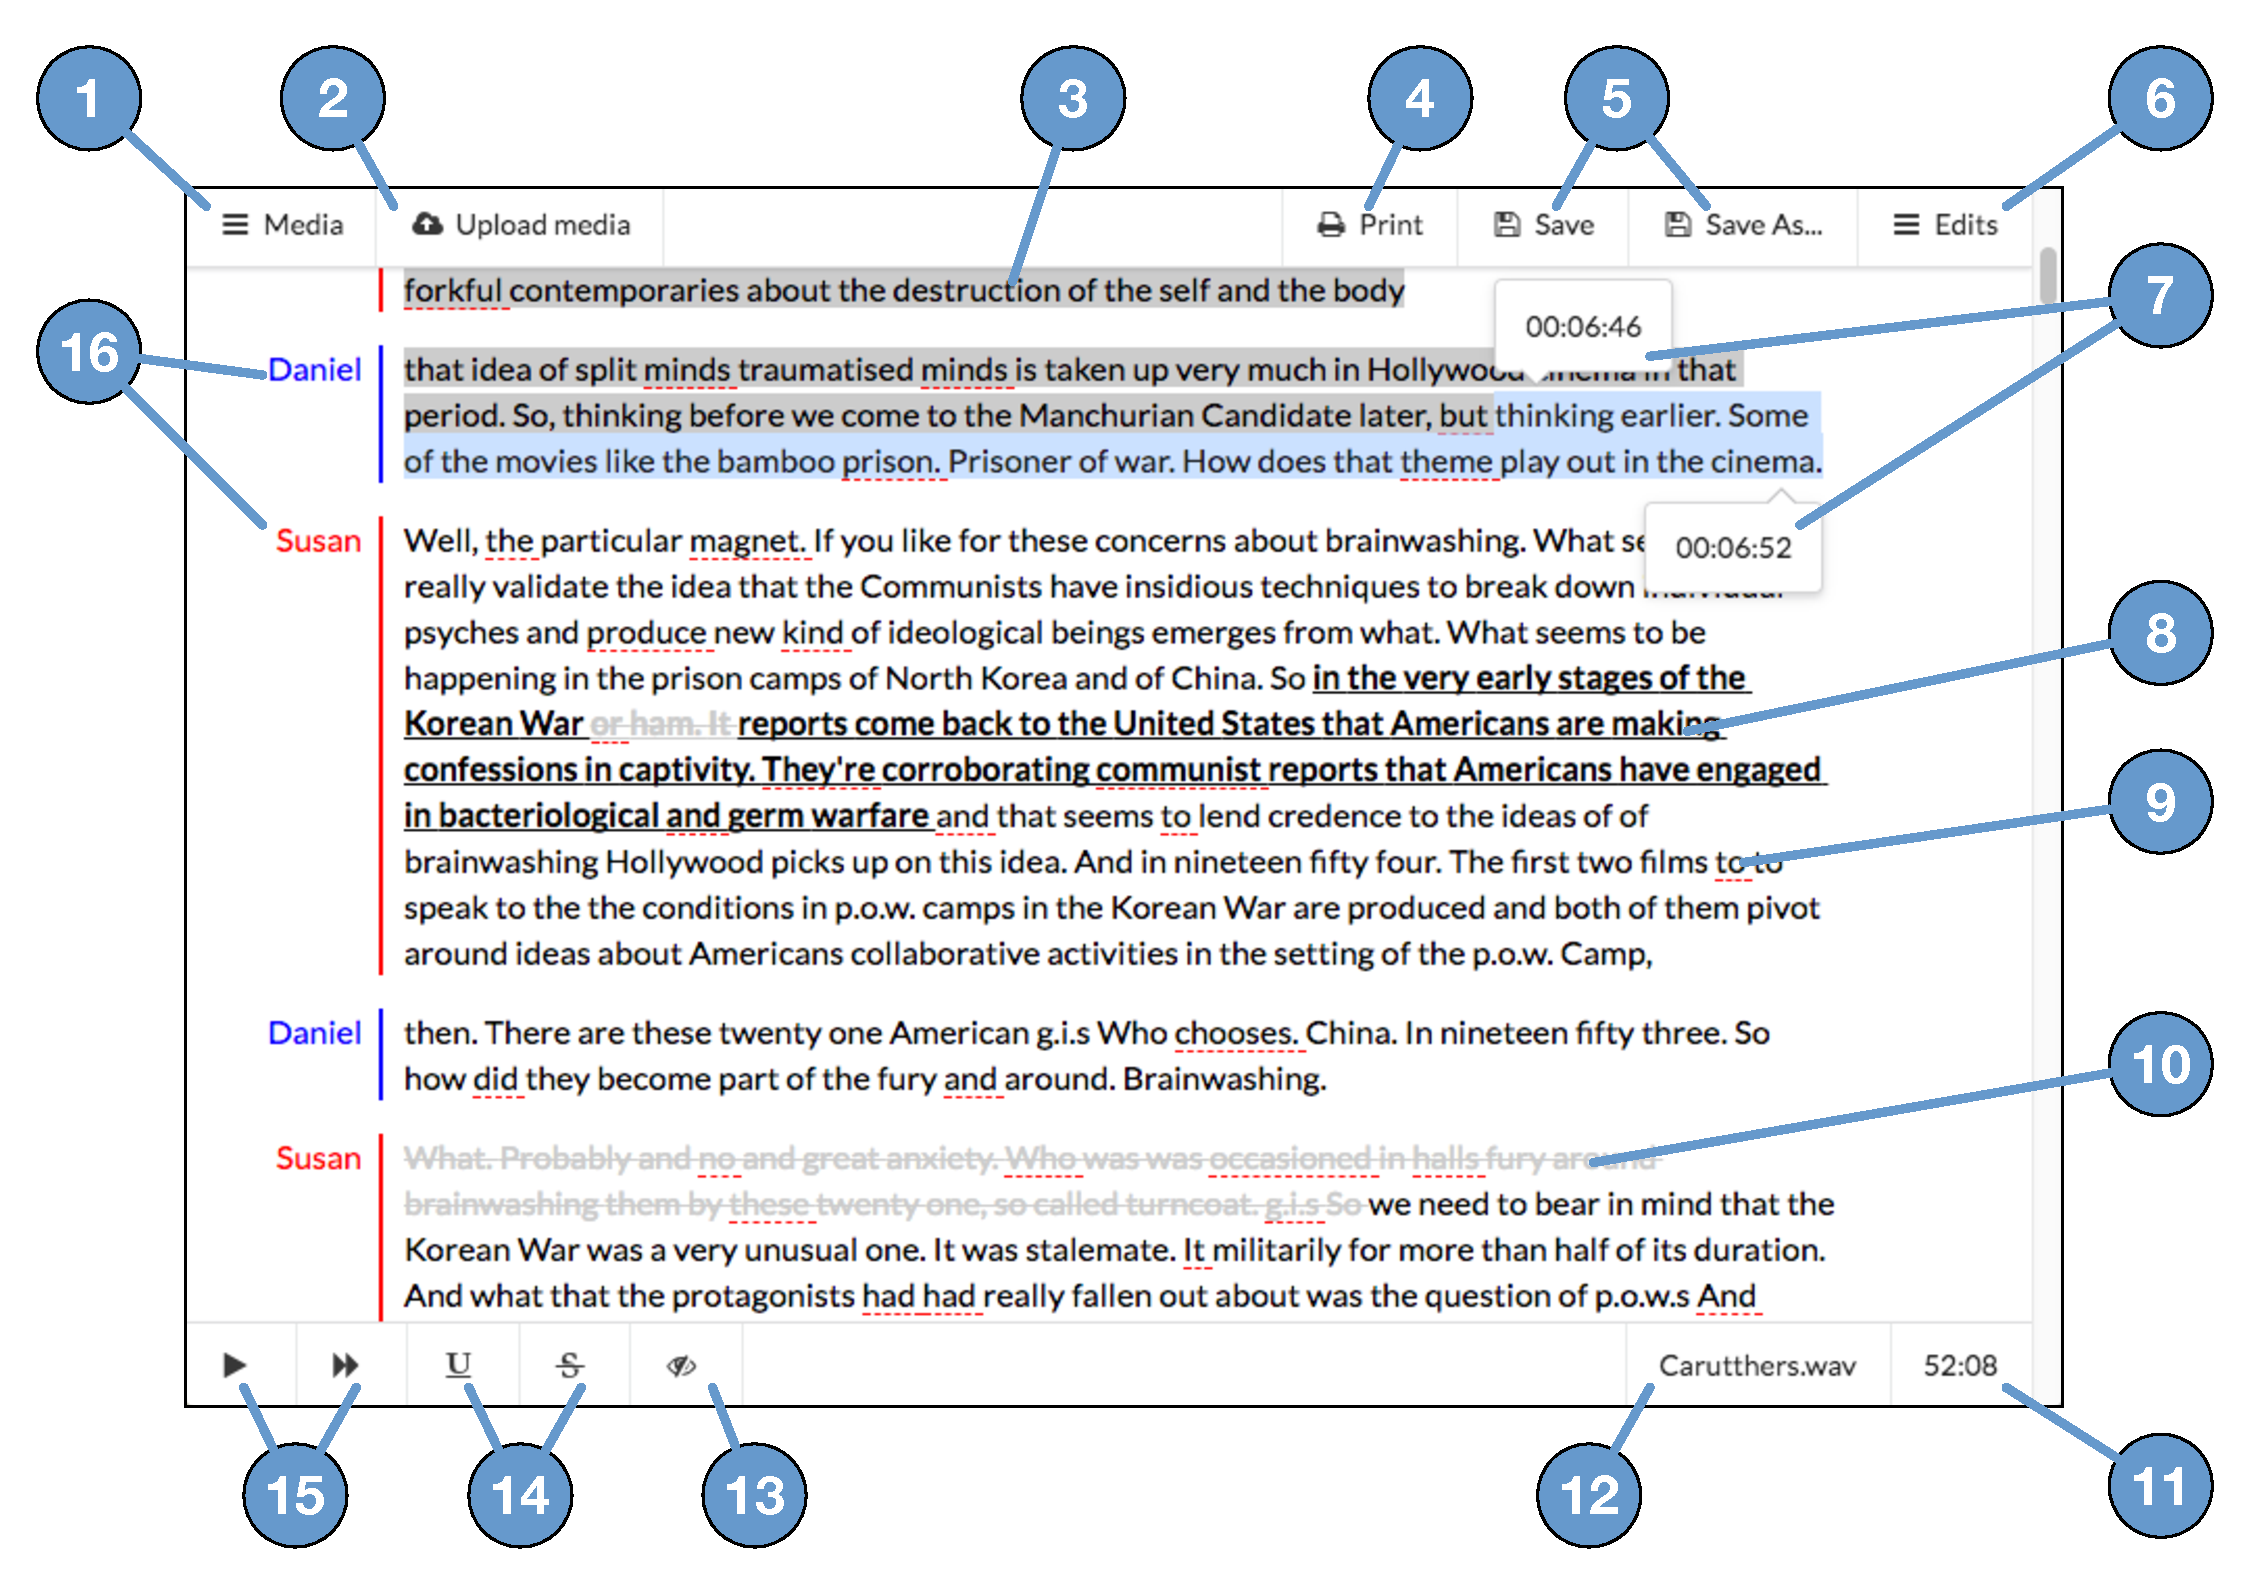
\includegraphics[width=\columnwidth]{figs/discourse-interface-labelled.pdf}
  \caption[User interface of the screen-based semantic speech editor.]{User interface of the screen-based semantic
    speech editor, which features 
    media storage (1),
    media upload (2),
    highlight of the current playback position (3),
    printing the transcript (4),
    saving edits and corrections to transcript (5),
    edit storage and export (6),
    displaying timestamps of the current selection (7),
    underlining words (8),
    confidence shading (9),
    strikethrough of words (10),
    display of edited audio duration (11),
    name of current asset (12),
    show/hide strikethrough (13),
    underlining/strike buttons (14),
    playback buttons (15)
  and speaker diarization (16)}
  \label{fig:dialogger-interface}
\end{figure}

We added a double-speed playback feature to allow faster than real-time listening, and a ``save-as'' feature to allow
multiple edits of the same material.  We implemented this by using collapsible sidebars to separate the original
``media'' on the left, from the modified ``edits'' on the right (see Figure~\ref{fig:download-pdf}).  We also included
speaker diarization using a label and line down the side of each paragraph, coloured by gender, and included confidence
shading using a dotted red underline to match the style of word processors.

\begin{figure}
  \centering
  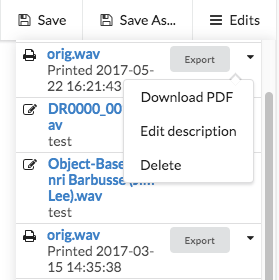
\includegraphics[width=0.4\columnwidth]{figs/discourse-download-pdf.png}
  \caption[Close-up of the edits sidebar of the screen-based semantic speech editor.]{Close-up of the edits sidebar of
  the screen-based semantic speech editor, showing a button to export audio, and a dropdown menu with the option to
download a PDF.}
  \label{fig:download-pdf}
\end{figure}


The screen interface included integrated playback, which allowed the user to listen to and navigate the audio while
they edit. The current playback position was shown in the text and the user could jump to a word by double-clicking it
on the transcript. Any edits made to the transcript were reflected in the audio.  The user could also correct any
mistakes in the transcript by editing the text as they would in a word processor.

%We updated the screen-based interface used in Chapter~\ref{chp:screen} to implement some of the
%changes suggested by our findings.
%The previous screen-based system is shown in Figure~\ref{fig:interface} on page \pageref{fig:interface}, and the
%updated interface is shown in Figure~\ref{fig:dialogger-interface} on page \pageref{fig:dialogger-interface}.
%The two major differences are that underline and strikethrough are used instead of drag-and-drop, and that only one
%recording can be edited at any one time.

%We replaced drag-and-drop with an underline/strikethrough method for three reasons.  Firstly, we found that there was
%not enough room to handle large clips, which was what most users were interested in.  Secondly, we found that users
%mostly used the tool for rough editing, so weren't interested in mixing different recordings together.  Finally, we
%wanted the edit scheme to match our paper-based interface, as this would allow us to compare the different modalities
%side-by-side, rather than different edit techniques.

%There were many other smaller changes we made to the interface. We added double-speed playback to allow users to listen
%faster than real-time, as requested by participants in our previous experiment. Previously, users could only make a
%single edit per project. For the updated version,


%We included speaker diarization using a line down the side of each paragraph, coloured by gender and with a label, and
%included confidence shading using a dotted red underline to indicate low confidence in order to match the style of word
%processors.

%\subsubsection{System description}

%Users can login using their normal BBC account. They are then presented with the edit screen, which
%has hidden sidebars on the left and right. Media that is uploaded is stored on the left-hand side, and any edits are
%stored on the right-hand side. Edits can be exported either as an EDL or as an edited audio file. Users can only edit
%one recording at a time, and multiple recordings must be mixed together at a later stage. Speakers are shown by a line
%on the left of each paragraph, and any words with a low confidence are underlined with a dotted red line.


\section{Evaluation methodology}\label{sec:paper-method}

The objective of our second study was to discover whether professional radio producers could use PaperClip as part of
their workflow, and to compare how the workflow was affected by PaperClip and our screen interface.  To find out, we
ran a within-subjects qualitative user study in which we tested radio producers editing speech recordings under three
different conditions:

\begin{enumerate}[label=C\arabic*.]
  \item PaperClip digital pen interface
  \item Screen interface
  \item Normal printed transcript
\end{enumerate}

We did not want to test the impact of the transcript itself, but rather the impact of the interface that was used to
interact with the transcript. Therefore, all three conditions used a transcript generated by the same ASR system,
developed by the BBC. Our ASR used the Kaldi toolkit\footnote{\url{http://kaldi-asr.org/}} and was trained on
television recordings.  The normal printed transcript acted as a control. It included speaker labels and timestamps,
but did not use the PaperClip layout or Anoto dot pattern.

We recruited eight radio producers from the current affairs, science and documentaries teams in BBC Radio.
Table~\ref{tab:participants} lists the participants and their self-reported professional experience and the department in
which they work.
Only one of the
participants overlapped with our first study in Section~\ref{sec:paper-requirements}.  As producers are very busy, we
designed our study to take less than a day to complete. Despite this, it took us 12 months to recruit the participants
and collect the data as producers often cancelled or re-arranged due to their demanding role.

\begin{table}[h]
  \centering
  \begin{tabular}{l l l}
      \hline
      \textbf{ID} & \textbf{Experience} & \textbf{Department} \\ %& \textbf{Computer literacy} \\
      \hline
      P1 & 13 years & Current affairs \\%& Medium  \\
      P2 & 16 years & Documentaries   \\%& Low     \\
      P3 & 8 years & Current affairs \\%& High    \\
      P4 & 10 years & Science         \\%& High    \\
      P5 & 18 years & Current affairs \\%& Low     \\
      P6 & 16 years & Current affairs \\%& Medium  \\
      P7 & 28 years & Documentaries   \\%& Medium  \\
      P8 & 20 years & Science         \\%& Low     \\
      \hline
  \end{tabular}
  \caption{Evaluation study participant demographics.}
  \label{tab:participants}
\end{table}

%To compare the paper and screen interfaces, we designed and conducted a user study.  The objective of our study was to
%see whether professional radio producers could use a paper-based semantic speech editing interface as part of their
%workflow, and to understand how paper-based and screen-based interfaces differently affected this process.

%\subsection{Design and procedure}
%We ran a within-subjects user study in which we tested radio producers editing speech recordings under three different
%conditions: a digital pen interface, a screen interface and a normal printed transcript. The printed transcript acted
%as a control and was inactive, in the sense that it did not make use of the Anoto dot pattern technology.  The
%transcripts for all three conditions were generated by the same speech-to-text system.


%We recruited professional radio producers exclusively from BBC Radio so that we could take advantage of the access 
%available to us. We recruited participants by sending an invitation by email to the current affairs, science and
%documentaries teams in BBC Radio.  Through this, we recruited eight participants who had between 8 and 28 years
%experience of professional radio production, with a mean average of 16 years experience.

%%TODO Talk about length of recruitment, difficulty in completing study

%We asked each participant to provide audio recordings from three recent interviews they had made, so we could use
%content that was genuine and fresh in their mind. We set a minimum duration of 20 minutes for each recording, as we
%found in the study in Chapter~\ref{chp:screen} that there was not much advantage in using transcripts for
%short recordings.

\subsection{Protocol}

The protocol for our study had three stages.

\paragraph{Stage 1: Training}

Firstly, the participant was briefed on the study and asked to sign a consent form.  The participant used a test
recording to perform a scripted series of tasks that used all of the features of each interface.  This allowed them to
use and experience all of the features for themselves. The participant was then given an opportunity to ask questions
and become familiar with each interface until they felt comfortable with using them.

\paragraph{Stage 2: Observation}

The participant completed three editing tasks, each under one of the three conditions (C1, C2 or C3).  The order of
conditions was balanced to avoid carryover effects.  We designed the experiment so that the editing tasks
overlapped with the work the producers already needed to do. This ensured that the tasks were genuine and part of a
real production.  The participant provided three recent speech recordings that they needed to edit so that the content
was fresh in their mind.  We needed to use different recordings for each condition, but we asked the participant to
choose recordings from the same programme to ensure they were as similar as possible.  In Chapter~\ref{chp:screen}, we
found that there was no benefit in using transcripts for short recordings, so each recording was at least 20 mins in
length. 
 
The investigator observed the task, made written notes about their behaviour, and logged the duration of each audio
file and the time taken to edit it, excluding any interruptions.  Items of interest at this stage included editing
workflow, tools used, data generated, usability challenges and problems, navigation and edit actions, time taken to
complete tasks, unexpected reactions and unanticipated usage. During any ``down-time'', we conducted ad hoc, in situ
interviews to clarify the process and any decisions that were made.  The observation took place at the participant's
normal work environment, which in all cases was a desk in an open plan office.  We considered recording the task using
a video camera, but due to the open-plan nature of the offices, there were insurmountable issues with privacy and
information security.

After each task, the participant filled out a questionnaire to measure the usefulness and usability of the interface,
using the Perceived Usefulness scale \citep{Davis1989} and the Software Usability Scale (SUS) \citep{Brooke1996},
respectively.  After completing all three tasks, the participant was asked to select which system they would prefer to
continue using.

%The second stage of the study was observing the participant whilst they edited three different recordings, each under
%one of the three conditions.  The order of the conditions was counterbalanced to avoid carryover effects. 

%During the observation, the investigator sat beside the participant and made written notes detailing their behaviour
%and noting anything of interest. If the participant had any `down-time', the investigator used this to clarify
%anything they didn't understand.  Items of interest at this stage included editing workflow, tools used, data
%generated, usability challenges and problems, navigation and edit actions, time taken to complete tasks, unexpected
%reactions and unanticipated usage

%During each task, the experimenter kept track of how long it took the participant to complete the task, excluding any
%time not spent on the task at hand (e.g. phone calls, making tea) and the length of each recording being
%edited.

%%TODO What was the expected result?

%After each task was completed, the investigator asked the participant to fill out a questionnairre to measure the
%usefulness and usability of the interface. We chose to use Perceived Usefulness \citep{Davis1989}, shown in
%Table~\ref{tab:perceived-usefulness}, and the Software Usability Scale \citep{Brooke1996}, shown in Table~\ref{tab:sus}.
%Photographs were taken of the paper annotation and work environment, with the participant's permission.

%\begin{table}
  %{\small
    %\begin{tabular}{ | l | }
      %\hline
      %Using this system in my job would enable me to accomplish tasks more quickly. \\ \hline
      %Using this system would improve my job performance. \\ \hline
      %Using this system in my job would increase my productivity. \\ \hline
      %Using this system would enhance my effectiveness on the job. \\ \hline
      %Using this system would make it easier to do my job. \\
      %\hline
    %\end{tabular}
  %}
  %\caption{Perceived usefulness questionnaire \citep{Davis1989}}
  %\label{tab:usefulness}
%\end{table}

%\begin{table}
  %{\small
    %\begin{tabular}{ | l | }
      %\hline
      %I would find this system useful in my job. \\ \hline
      %I think that I would like to use this system frequently. \\ \hline
      %I found the system unnecessarily complex. \\ \hline
      %I thought the system was easy to use. \\ \hline
      %I think that I would need the support of a technical person to be able to use \\
      %this system. \\ \hline
      %I found the various functions in this system were well integrated. \\ \hline
      %I thought there was too much inconsistency in this system. \\ \hline
      %I would imagine that most people would learn to use this system very quickly. \\ \hline
      %I found the system very cumbersome to use. \\ \hline
      %I felt very confident using the system. \\ \hline
      %I needed to learn a lot of things before I could get going with this system \\
      %\hline
    %\end{tabular}
  %}
  %\caption{Software usability scale questionnaire \citep{Brooke1996}}
  %\label{tab:sus}
%\end{table}

%After completing all of the tasks, we asked the participant to fill out a form to measure user preference. The form
%asked

%\textit{``Of the three systems you have just tried, which of them would you most prefer to continue
%using?''}

%and had a checkbox for each of the three interfaces.

%%TODO What is the expected result?

\paragraph{Stage 3: Interview}

The investigator conducted a semi-structured interview using the following questions.  The order of questions 2--4 was
adjusted to match the order in which the conditions were presented to the participant.  An audio recording was made of
the interview for later analysis.

%For the final stage of the study, the experimenter performed a semi-structured interview with the participant. This
%gave the participant the opportunity to discuss each of the three conditions in detail and compare them directly. An
%audio recording was made of the interview, which was used to perform in-depth analysis.

%We asked the participant the following questions:

{\singlespacing
  \begin{enumerate}
    \item Can you please describe your existing process for editing audio?
    \item What did you like or dislike about the pen-based system?
    \item What did you like or dislike about the screen-based system?
    \item What did you like or dislike about using normal paper?
    \item Overall, which of these systems would you most prefer to continue using, and why?
  \end{enumerate}
}

%The final question gave the participant an
%opportunity to explain their decision made at the end of Stage 2.

%The first question was included to understand more about the participant's current approach, in case that affected
%their preferences or usage of the systems.  The order of questions 2--4 were adjusted to match the order in which the
%conditions were presented to the participant.


\subsection{Analysis}

We transcribed the interview recordings and corrected the words manually using the screen interface described in
Section~\ref{sec:paper-screen-design}.  Using grounded theory \citep{Silverman2016}, the investigator then openly coded
the transcripts and observation notes using \textit{RQDA} \citep{RQDA}, which produced 229 initial codes. The
investigator then used \textit{FreeMind} mind-mapping software to group the codes into categories, and the categories
into themes.

The time taken to edit an audio file depends upon its length.  As recommended by \citet{Dewey2014}, we divided the edit
speed of each task by the audio file duration to calculate the ``normalised task completion time''.  Following the
procedures described in \citet{Davis1989,Brooke1996}, we converted the questionnaire data measuring the usefulness and
usability into individual scores between 0 and 100. We used within-subjects one-way ANOVA \citep{Rouanet1970} to test
for differences between the systems in the relative edit time, perceived usefulness and usability (SUS) metrics.  For
the system preference data, we simply report the count of the preferences for each system.

%We performed both qualitative and quantitative analysis on the data we collected during our study.

%For the qualitative analysis, we transcribed all of the audio recorded during the interviews by using our screen-based
%interface to run speech-to-text and then correcting the words manually. This process produced approximately 23,000
%words of transcripts. Using grounded theory, the principal investigator then openly coded the transcripts and
%observation notes using the RQDA software package. This produced 229 different codes. The principal investigator used
%mind-mapping software to group these codes into 15 categories, then grouped the categories into three high-level
%themes. For each category, we extracted representative quotes from the interviews to illustrate the key points made.

%During the study, we collected data about task duration, system preference, usefulness and usability.  We plotted the
%task duration measurements against the duration of the audio being edited. For each condition, we drew the linear
%regression to see how the edit time is affected by longer or shorter recordings, and to compare the the edit time of
%the three conditions.

%The questionnaire data measuring the usefulness and usability were individually converted into
%scores between 0 and 100.  This follows the procedure described in \citet{Davis1989} for usefulness, and
%\citet{Brooke1996} for usability.  For the system preference data, we simply reported the count of the participants'
%preference for each system.

\section{Evaluation results}\label{sec:paper-results}

In this section, we will present the quantitative and qualitative results that emerged from the metrics, observation
notes and interviews in our evaluation study.  The themes and categories that resulted from the analysis of the
interview transcripts and observation notes are shown in Table~\ref{tab:paper-codes}.  We will start by looking at the
metrics and user preferences we gathered, before summarising the comments made by participants in each of the
categories and themes that emerged from the thematic coding process.

\begin{table}[p]
  \centering
  {\small
    \begin{tabular}{l l l} %p{0.18\linewidth}|p{0.2\linewidth}|p{0.5\linewidth}|}
      \hline
      \textbf{Theme} & \textbf{Category} & \textbf{\# codes} \\ \hline
      \multirow{8}{*}{Editing}
      & Collaboration & 15 \\ %\cline{2-3} %Easier with digital representation (screen), Remotely, Compare notes with presenter, Timecodes or page/line numbers for reference, Side-by-side comparison, Google Docs, Share new material with presenter, With third-party institutions \\ \cline{2-3}
      & Annotation & 16 \\ %\cline{2-3} %Colours, Highlight, Summary (auto?), Star, Labelling/numbering (auto?), Freehand, Speaker names, Music information \\ \cline{2-3}
      & Location & 11 \\ %\cline{2-3} %Thinking space, Away from desk/screen, Downtime - plane/train/bus, Quieter, Concentration \\ \cline{2-3}
      & Export & 7 \\ %\cline{2-3} %Transcript and annotations in DAW, Move selections to different track, Spaces between exported clips \\ \cline{2-3}
      & Pen & 35 \\ %\cline{2-3} %Narrow margin, Could be lost/broken, No correction, Cost, Can't draw freehand, only strike/underline, Note digitisation, Poor ergonomics, Desired gestures, Simplicity/lack of functionality, Lack of undo (same as normal pen), Must be precise, Easier to edit without interrupting playback, Higher edit precision, Permanency increased decisiveness \\ \cline{2-3}
      & Technique & 24 \\ %\cline{2-3} %Re-ordering and mixing (cut/paste), Pull out good bits, Remove bad bits, Rough edit first, Check nothing's been missed, Taking too much at early stage, Simultaneous correct and edit, Top and tail, Paper edit only (no listen), Multiple iterations (re-print) \\ \cline{2-3}
      & Decisions & 12 \\ %\cline{2-3} %Must be made in real-time, Easier to decide with paper, Simultanous listening/editing easier on paper \\ \cline{2-3}
      & Interface & 21 \\ \hline %Familiarity, Learning curve, Auto-labelling?, Limited options (faster?), All in one place, Editing large chunks, Training/cheatsheet, One of many different systems \\ \hline
      \multirow{4}{*}{Transcript}
      & Paper & 15 \\ %\cline{2-3}%Multiple windows/tabbing, Can't print on location, Quantity of paper (high), Takes time to print, Physicality, touch, Better, faster comprehension, Use of finger/pen to navigate, Bimodal reading/listening is better, Improves memory \\ \cline{2-3}
      & Accuracy & 17 \\ %\cline{2-3} %Use of memory affects threshold, Field recordings, Affects speed, Punctation (distracting), Good enough, Speaker diarization, Affects amount of listening, Accents, Noise, Affects edit resolution, Doesn't show umms/breaths \\ \cline{2-3}
      & Generation & 10 \\ %\cline{2-3} %Skipping/paraphrasing, Clerical job, Simultaneously making edit decisions in head, Takes too long, Third-party, overnight, Turnaround time, Question marks, Cumbersome/tedious \\ \cline{2-3}
      & Correction & 12 \\ \hline %Depends on length (don't need to for shorter), Not on paper, Fix repeat errors, For giving to other people, PasB transcript \\ %\cline{2-3}
      % & Technique & TV (thumbnails, expense), Search archive material, Compare and orientate other recordings from programme \\ \hline
      \multirow{3}{*}{Listening}
      % & Speed & Discourse x2 playback hard to understand, Use memory to skip, Faster with transcript \\ \cline{2-3}
      & Navigation & 8 \\ %\cline{2-3} %Can use finger as cursor on paper, Jumping around (easier with DAW), Timestamps, Reading ahead, Space bar to start/stop \\ \cline{2-3}
      & Criteria & 14 \\ %\cline{2-3} %Intonation, Works on paper, not on audio, Transcript accuracy, Do clips work on their own/together?, Sound effects (e.g. thunder), Umms, Breaths, Does edit work?, Is transcript correct? \\ \cline{2-3}
      & Technique & 12 \\ \hline %Process/reinforce information, Fine editing, 'Listening is editing', Mental buffering during de-umming \\ \hline

    \end{tabular}
  }
  \caption{Themes, categories and number of codes that resulted from the quantitative analysis of the interviews and
  observations.}
  \label{tab:paper-codes}
\end{table}


\subsection{Metrics}\label{sec:paper-metrics}

\begin{figure}[p]
  \centering
  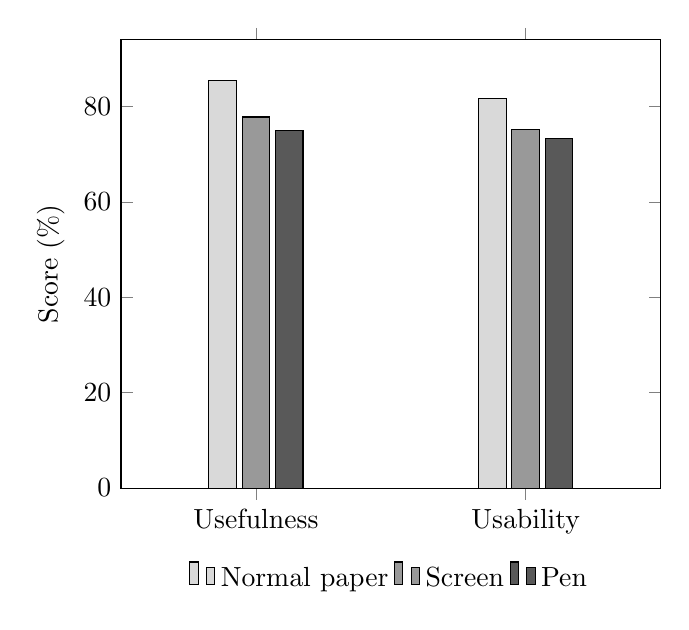
\begin{tikzpicture}
    \begin{axis}[
      ybar,
      ymin=0,
      enlarge x limits=0.5,
      legend style={at={(0.5,-0.15)},anchor=north,legend columns=-1,draw=none},
      ylabel={Score (\%)},
      symbolic x coords={Usefulness, Usability},
      xtick=data,
      %nodes near coords,
      %nodes near coords align={vertical},
      %every node near coord/.append style={font=\footnotesize},%xshift=-15pt,yshift=-3pt,anchor=east,font=\footnotesize},
      ]
      \addplot[fill=black!15] coordinates {(Usefulness,85.42) (Usability,81.67)};
      \addplot[fill=black!40] coordinates {(Usefulness,77.78) (Usability,75.21)};
      \addplot[fill=black!65] coordinates {(Usefulness,75.00) (Usability,73.33)};
      \legend{Normal paper, Screen, Pen}
    \end{axis}
  \end{tikzpicture}
  \caption[Mean average scores for usefulness and usability.]{Mean average scores for usefulness and usability. There
  is no statistically significant difference between the scores.}
  \label{fig:pen-useful-usable}
\end{figure}

When asked which system they would prefer to continue using, four of the eight participants chose PaperClip, two (P3
and P6) chose the screen interface and two (P1 and P4) chose the normal paper transcript.  Although it did not include
any semantic editing functionality, P1 and P4 said they preferred the normal paper transcript as it allowed them to use
their existing workflow and tools, which they found easiest and most comfortable.  This demonstrates that ASR
transcripts themselves are beneficial to radio production.

Figure~\ref{fig:pen-useful-usable} shows the mean average scores of the usefulness and usability of the three systems.
%For the SUS metric, the mean ratings for PaperClip, screen interface and normal paper were 73\%, 75\% and 82\%, and
%for perceived usefulness they were 75\%, 78\% and 85\%, respectively.
A one-way within-subjects ANOVA showed that there was no statistically significant difference between the systems for
usefulness [$F(2,14)=0.788, p>0.05$], nor usability [$F(2,14)=1.068, p>0.05$].  Using the SUS grading system from
\citet{Sauro2016}, we can compare the usability score to other systems in general.  The grades for normal paper, screen
and pen were A, B and B--, respectively, which shows that all of the tools appear to perform well overall.

%The SUS grading system \cite{Sauro2016} scored the
%usability for the normal paper, screen and digital pen as A, B and B--, respectively. This shows that compared to other
%interfaces in general, they seem to work well.

For each task, we divided the edit time by the audio duration to calculate the relative edit time.  The screen and
normal paper interfaces had the same mean relative edit time ($\times 0.99$ real-time), but PaperClip was 16\% faster
($\times 0.83$ real-time).  This was surprising, as we expected the screen interface to be faster than both the pen and
normal paper due to its integrated playback feature.  However, a one-way within-subjects ANOVA did not find any
statistically significant difference [$F(2,14) = 0.931, p > 0.05$].

The metrics results show that although half of participants preferred the PaperClip interface and it had the fastest
relative edit time, it was rated least useful and least usable. 
To try to better understand these ratings, we now turn to the interview and observational
data.

%\subsection{Metrics}

%% Preference
%\subsubsection{Preference}\label{sec:pen-preference}

%Directly after each participant completed the three tasks, we asked them to select which of the interfaces they would
%prefer to continue using. As shown in Figure~\ref{fig:pen-preference}, four of the eight participants chose the pen
%interface, with two (P3 and P6) choosing the screen and two (P1 and P4) choosing the normal paper transcript.

%Although we expected that participants may be split between the paper and screen interfaces, we did not expect anybody
%to prefer the normal transcript, as it did not include any semantic editing functionality.  Both P1 and P4 preferred
%the normal paper transcript because it allowed them to continue to use their existing workflow, which they found
%easiest and most comfortable.

%\textit{``I can retro fit it into the way that I currently work most easily because it is essentially the same way that
%I do work, but with an extra paper transcript.''} (P4)

%%\textit{``That is the most natural to me that is what I felt most comfortable with doing.''} (P1)

%The paper transcript allowed participants to use their existing tools, which they used regularly, and therefore could
%achieve the same objective without having to learn how to use new systems or interfaces. Although the normal printed
%transcripts did not include any features other than the transcript itself, the fact that two of the producers would
%prefer to use it demonstrates the value of the transcript itself and the familiarity with the toolset.

%\begin{figure}[p]
  %%\begin{subfigure}[b]{0.5\textwidth}
    %\centering
    %%\resizebox{\linewidth}{!}{
      %\begin{tikzpicture}
        %\begin{axis}[
          %ybar,
          %ymin=0,
          %enlarge x limits=0.5,
          %legend style={at={(0.5,-0.15)},anchor=north,legend columns=-1},
          %ylabel={Count},
          %symbolic x coords={Paper, Screen, Normal},
          %xtick=data,
          %nodes near coords,
          %]
          %\addplot coordinates {(Paper,4) (Screen,2) (Normal,2)};
        %\end{axis}
      %\end{tikzpicture}
    %%}
    %\caption{System preference}
    %\label{fig:pen-preference}
  %%\end{subfigure}
  %%~
  %%\begin{subfigure}[b]{0.5\textwidth}
    %%\centering
    %%\resizebox{\linewidth}{!}{
      %%\begin{tikzpicture}
        %%\begin{axis}[
          %%ybar,
          %%ymin=0,
          %%enlarge x limits=0.5,
          %%legend style={at={(0.5,-0.15)},anchor=north,legend columns=-1},
          %%ylabel={Edit time/Audio duration},
          %%symbolic x coords={Paper, Screen, Normal},
          %%xtick=data,
          %%nodes near coords,
          %%]
          %%\addplot coordinates {(Paper,0.8295) (Screen,0.9890) (Normal,0.9867)};
        %%\end{axis}
      %%\end{tikzpicture}
    %%}
    %%\label{fig:pen-speed}
    %%\caption{Mean edit time, relative to the duration of the audio being edited. There is no statistically significant
    %%difference between the times.}
  %%\end{subfigure}
  %%\caption{Comparison of metrics}
%\end{figure}

%% Usefulness and usability
%\subsubsection{Usefulness and usability}


%% calculated using http://www.statisticslectures.com/calculators/anovawithin/index.php
%Figure~\ref{fig:pen-useful-usable} shows the mean average scores of the usefulness and usability of the three systems.  We
%performed one-way within-subjects ANOVA on the usefulness and usabilty scores. This found that there were no
%statistically significant differences between the three systems for usefulness [$F(2,14)=0.788, p>0.05$], nor usability
%[$F(2,14)=1.068, p>0.05$].

%We can compare the usability of our three systems to other systems in general by using the SUS scores from 
%previous studies. These have been collected and reviewed in \citet{Sauro2016}, which also includes method to convert
%the SUS score into a representative grade between A and F.  The grades for normal, screen and pen were A, B and B--,
%respectively. This shows that, generally speaking, the tools seem to work well.

%Although there was no statistically significant difference, the higher scores received by the normal printed transcript
%are unexpected. This could imply that the semantic editing features offered by the screen and pen interfaces have a
%negative impact on the usefulness and usability of the system, although this was not supported by the qualitative
%results. It is also possible that participants scored the normal paper system higher as they felt more
%comfortable and familiar using their normal toolset rather than a prototype, as mentioned in
%Section~\ref{sec:pen-preference}.

%%Several participants felt as though the existing workflow was the most comfortable or easiest of the three conditions
%%we tested. P7 said that having a printed transcript was useful as an aide memoire.

%%\textit{``what I liked [about the normal paper] is that it's very similar to what I'm used to so there is familiarity''}
%%(P6)

%%Some participants preferred the normal printer paper transcript to either of the semantic editing interfaces, as it was
%%more familiar to them.

%% Speed
%\subsubsection{Speed}

%\begin{figure}[ht]
%\centering
%\begin{tikzpicture}
%\begin{axis}[
%legend pos=outer north east,
%legend cell align=left,
%xmin=0,
%ymin=0,
%xlabel={Audio length (mins)},
%ylabel={Edit time (mins)}]

%% NORMAL
%\pgfplotstableread{
%X Y
%30 30
%58 43
%32 23
%35 53
%28 35
%28 32
%47 62
%28 22
%}\normaltimes
%\addplot [only marks, mark = *, red] table {\normaltimes};
%\addlegendentry{Normal paper}
%\addplot [thick, red, forget plot] table[
%y={create col/linear regression={y=Y}}
%]{\normaltimes};
%%\addlegendentry{Normal trend}

%% SCREEN
%\pgfplotstableread{
%X Y
%37 24
%61 61
%30 30
%25 49
%26 31
%41 28
%37 37
%33 45
%}\screentimes
%\addplot [only marks, mark = square*, blue] table {\screentimes};
%\addlegendentry{Screen}
%\addplot [thick, dotted, blue, forget plot] table[
%y={create col/linear regression={y=Y}}
%]{\screentimes};
%%\addlegendentry{Screen trend}

%% PEN
%\pgfplotstableread{
%X Y
%12 9
%75 56
%31 17
%22 19
%27 27
%38 37
%33 33
%28 41
%}\pentimes
%\addplot [only marks, mark = diamond*, green] table {\pentimes};
%\addlegendentry{Pen}
%\addplot [thick, loosely dashed, green, forget plot] table[
%y={create col/linear regression={y=Y}}
%]{\pentimes};
%%\addlegendentry{Pen trend}

%\end{axis}
%\end{tikzpicture}
%\caption{Edit time versus audio duration for each condition, with linear regression plots.}
%\label{fig:pen-speed}
%\end{figure}

%Figure~\ref{fig:pen-speed} shows the edit time for each condition, plotted against the duration of the audio being
%edited.
%% calculated using http://www.statisticslectures.com/calculators/anovawithin/index.php
%We performed one-way within-subjects ANOVA on the relative edit time and did not find any statistically significant
%difference [$F(2,14) = 0.931, p > 0.05$], which may be due to the small sample size.  We have also plotted the linear
%regression to show the trend for each condition. The gradient of the lines are comparable, which indicates that the
%audio duration affects the edit time similarly for each condition.  If we divide the edit time by the audio duration,
%we can calculate the mean relative edit time which is 0.83 for the pen, 0.99 for the screen and 0.99 for the normal
%paper.

%%The mean edit time per minute of input audio was 59.2, 59.34 and 49.77 seconds for the normal paper, screen and pen
%%interfaces, respectively.

%The screen and normal paper interfaces had the same mean relative edit time, but the pen was faster by 16\%.  This was
%surprising, as we expected the screen interface to be faster than both the pen and normal paper due to its more
%powerful navigation features. As discussed in Section~\ref{sec:paper-edit-decisions}, some participants found that the
%simplicity of the pen interface allowed them to make edit decisions faster. This matches with the data, but the results
%are not statistically significant so more investigation is required.

\subsection{Editing}


% ======================= DECISIONS


%It closely replicates the existing
%workflow of some producers who already work on paper, which may have helped make some of the participants more
%comfortable.

\subsubsection{Decisions}
Participants P4, P5 and P8 reported that they could make editorial decisions faster and more easily on paper compared
to the screen because of the reduced functionality of the interface, uninterrupted playback of the audio, natural edit
gestures and faster reading speed.  P4 said that the lack of correction features in PaperClip allowed them to
edit faster than the screen, as it didn't interrupt their flow.

\textit{``I liked how it limited my options, [...]
  because with the screen I think what slowed me down
  was the fact that I could be
  %approaching it in different ways [by]
  %And so I was trying to approach it in several ways
  [...] simultaneously correcting the transcript and trying to edit the content. [...]
  %%and that's probably why it took as long.
  With the pen, I couldn't, so there's no point stopping. [...]
  %also because I had a good
  %interviewee then I could just listen in real time. I knew roughly what I wanted him to say and 
  %I knew roughly where the good points were,
  %so I could just listen through and then just go `no, yes, no, yes'.
  I don't think I've ever done an edit that fast, where it was literally real-time.''} (P4)

%When an edit was made using the screen interface, the playback would pause while the audio edits were applied, and the
%playback had to be manually restarted. With the pen interface, participants used a separate device to play the audio so
%the playback was not affected.  P4 and P8 said that this allowed them to edit with uninterrupted playback.

%\textit{``On the screen [...] I couldn't listen and edit at the same time, whereas I could listen and edit with the
%pen.''} (P8)

%reading speed
P2 and P5 reported that they could process the information faster when reading on paper compared to the screen. P5 said
that when using the screen, they would select more than necessary because their decision-making couldn't keep up with
the audio.

%\textit{``I think you do read slower on screen.''} (P2)

\textit{``The [screen] felt too quick and much harder to make a decision. It was like
  %`oh sod it
  `just keep everything', because you don't want to miss something.''} (P5)

P8 said they felt that the digital pen allowed them to be more precise with their edits than with the screen.  Although
the screen is just as precise, the digital pen can be used to start making a selection without knowing the endpoint.
This allows the producer to decide as they listen, which may give a feeling of better control over precision.


% =================== PEN

\subsubsection{Pen}

P5, P6 and P8 felt that the physicality of the PaperClip interface made it user friendly, intuitive and simple.

\textit{``It feels like you're working analogue, but you're actually working digitally. [...] It's nice to hold a pen
and go on real paper, which has the feel of every day life.''} (P7)
%\textit{``I do like a nice pen and paper I just do like to write stuff down and I'm quite scribbler.''} (P5)

The design of PaperClip forced users to select or delete content by drawing lines within strictly defined zones
that are interpreted literally. P3, P5, P7 and P8 said they did not like that they could not freely draw on the page and were
concerned about potential errors that could be introduced by straying outside of the boundaries.

\textit{``[PaperClip] doesn't have the convenience of paper, which is that there's no real rules [and] you can
write anywhere on the paper.''} (P3)

%\textit{``If you're sloppy, then you're going to get a squiggle in the wrong area.''} (P7)


%\textit{``[The pen felt] more accurate first time round and therefore maybe you only have to do two takes rather than
%several. [...] You could get more precision I think.''} (P8)

P3 and P6 said that they did not like that there wasn't any way to undo the edits using PaperClip. P6 suggested
that the lack of undo functionality may force them to be more decisive.

\textit{``It's harder to say `oh no I've changed my mind, I want to go back', so you almost have to be much more
decisive, which maybe is a good discipline.''} (P6)

%\textit{``Presumably the pen is very expensive is it?''} (P2)

P2, P3, P5 and P7 were interested in the cost of the pen as they were concerned about losing or breaking a potentially
valuable item.  P3 and P5 noted that other valuable items, like headphones and recorders, are normally shared amongst
producers in a team but that they often disappear or get broken.

%\textit{``...not an issue until you lose the pen. You'll probably have to have it on a chain around your neck, like my
%glasses nowadays.''} (P7)

\textit{``Pens which are not connected to anything will go missing and get lost.
  %umm so if that becomes part of your
  %standard workflow. is Everybody going to have their own pen? at the moment. We don't have a system where everyone has
  %their own headphones. This
  [We have a] constant problem with headphones going missing in this department [...]
  %which is a similar technology
and the solution is that the headphones are actually bolted to the desks.''} (P3)

Often transcripts can be very long, so printing them requires a large amount of paper. P2 used a long recording
for the experiment that required over 50 sheets of paper, which they said was \textit{``quite wasteful''}.
The Anoto system also requires access to a colour laser printer.
This is not usually a problem in an office environment, but can be an issue when travelling, or when
working from home.

%\textit{``50 sheets of paper is rather a lot, yeah --- quite wasteful.''} (P2)

% ==================== COLLABORATION


%\textit{``Obviously, working from transcripts makes it easier to compare notes and sort of work as a team''} (P6)

%\textit{``Whoever the presenter is and myself - we would have heard some of it and then we decide together on paper. As
  %they are writing the script, I'm editing the clips. I'm listening to it and sometimes I have to amend what we've
%decided on paper because it doesn't quite work. There's a sort of back and forth going on.''} (P6)

% PAPER

\subsubsection{Collaboration}
Radio producers work with a variety of people including presenters, assistant producers, contributors and
organisations.  P3, P6 and P7 said that transcripts make it easier to collaborate as they create a common reference
point that is easy to share and annotate.

\textit{``The way we're doing it is printing out our transcripts and we can all go `page 15' [...]
  %or you can use timecodes, but
there's a common reference, whereas if you're just doing audio it's harder.''} (P6)

The physical nature of paper allows people in the same room to hand around transcripts, point at words and lay pages
out. However, the digital nature of the screen means it can be used for remote collaboration. For example, P6 reported
that they use Google Docs to simultaneously write and edit the script remotely with the presenter.

%\textit{``Keeping it all on screen makes it much easier to share and be collaborative with people who are not in the
%same room.''} (P3)


\textit{``I think of the three, [the screen] has the most potential to be a collaborative thing. [...]
  %I'm not quite sure how
  %it would work out yet. [...]
  %%I don't know if you can share. and Everyone can compare versions.
  Maybe if you could have two scripts side by side to have my transcripts with my bits highlighted and the presenters,
with their bits highlighted.''} (P6)

%\textit{``I would say in that case if you're sharing with your presenters or contributors or production staff, then
  %you're going to be using the screen-based system. But you may have already used the pen to get to where you're
%getting.''} (P7)

% ============== LOCATION

\subsubsection{Location}
P1, P5, P7 and P8 said that they often prefer to work away from the office, such as at home, to help them focus and get
more work done.  P7 and P8 suggested that PaperClip was well-suited for travel, such as during commuting, which
may provide an additional opportunity to be productive in what would otherwise be considered downtime.  Although, P7
pointed out that the screen interface could be used on-the-road with a laptop and noise-cancelling headphones. 

%\textit{``I do go away from my desk. I find it useful to have thinking time away. [...] Sometimes I just like to have a
%break from the screen.''} (P1)

%\textit{``I'd probably spend a couple of days at home to get it into shape [because] it's quieter [...]
  %%. Not that this office is anywhere near as noisy as the last office. You can sort of get into a zone a bit,
  %so you can really really concentrate. You save travelling time, and
\textit{``With the pen you could do stuff on the train [...]
  %couldn't you, because you can edit on a train. That would be more accurate... easier then editing on a train.
or on a bus. You could do it anywhere as long as it's not too bumpy.''} (P8)

P5 said they did not enjoy spending too long sitting upright at their
desk, and P7 cited comfort as a factor in where they prefer to work.

\textit{``I would feel more comfortable with a nice digital pen and a sheet of paper sitting on a couch [...]
  %or something like that. Doing it then realising it's cut the audio already... Christ,
  You could do it in bed - that would really have your work-life balance sorted, wouldn't it?''} (P7)

% ============== TECHNIQUE
\subsubsection{Technique}
P1, P2, P6 and P8 reported that editing was an iterative process. P2 said this was because they are not sure what they
need in the early stages, so they select too much then reduce it later. P8 said that what they select, or how much they
select, depends on what was said in other interviews, and P1 said they often have to go back to re-edit clips in a
different way. 

%\textit{``I was just taking probably taking far too much as I'm perhaps not quite sure what I need from that
%interview.''} (P2)

%\textit{``Usually when it comes to making the programme it will turn out that I want to use a clip in a different way;
  %so I'll have to take the clip and add on a little bit, or get another piece from somewhere else that I wasn't
%expecting''} (P1)

%\textit{``For a documentary I would rough edit, put everything in order and edit once, edit twice and maybe a third
%time to refine it, until you get it to time.''} (P8)

%\textit{``Sometimes I take a break from the screen and just have a look to check there's no crucial clips of bits of
%audio I might want to use that I haven't put in the script.''} (P1)

P1, P6 and P8 reported that all three systems we tested were only suitable for the first iteration, known as a ``rough
edit'', because they were missing two features --- re-ordering and labelling. Re-ordering is used to to see and hear how
different clips from separate interviews would work together, and labelling is used to help the producer navigate,
organise and structure their content. 
%P5 used PaperClip's margin to write labels and mark questions, but
%these were not digitised or made available in the exported edit.
%,as shown in Figure~\ref{fig:p5-annotations}.

%\textit{``This paper edit stage is normally what I do just as a rough first thing to do. It's not for when I'm actually
%editing the clips''} (P1)

%\textit{``Doing a cut which jumps from three different interviewees who are talking about the same topic that seems
%like the next natural step''} (P3)

% MARKING SPECIAL REGIONS

P5 used annotations to segment and label the transcript (see Figure~\ref{fig:p5-annotations}), which helped to
structure the material.

\textit{``I was just labelling by summarising a paragraph in about two or three words --- just who is speaking and the
substance of it --- or maybe just putting a cue to say that was a question.''} (P5) 

\begin{figure}[h]
  \centering
  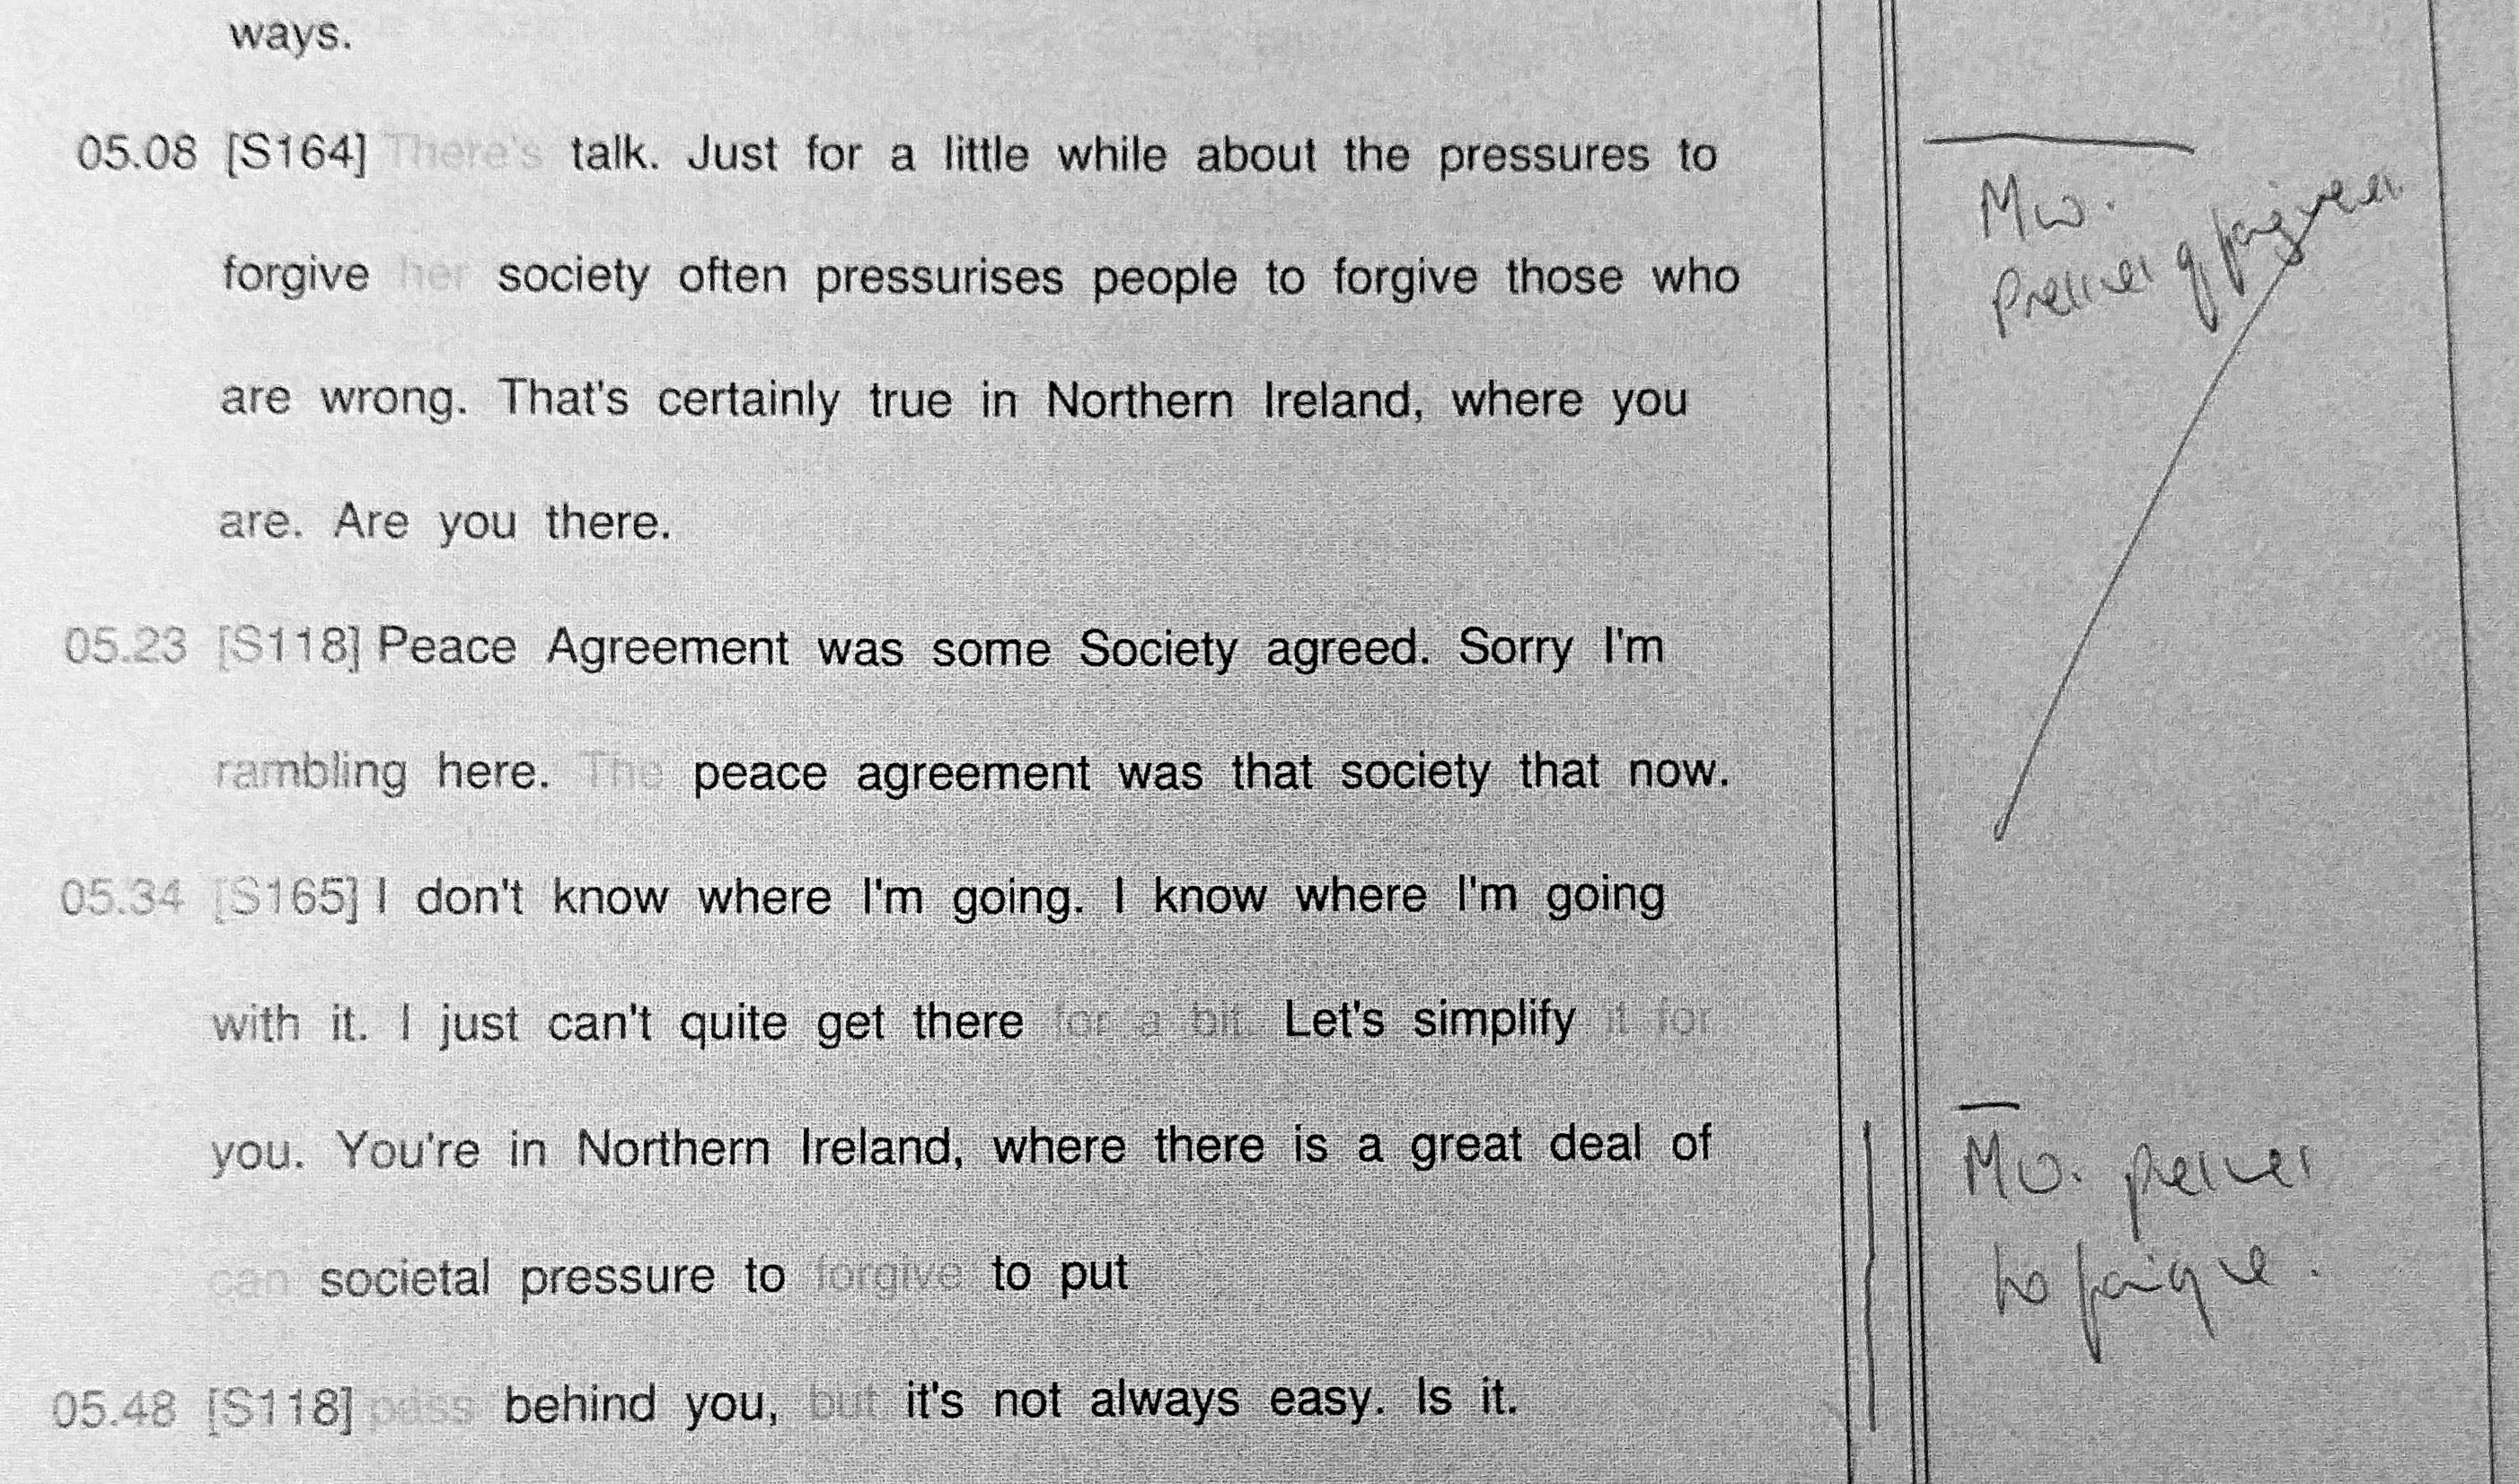
\includegraphics[width=\columnwidth]{figs/pen-annotations-p5-cropped-bw.jpg}
  \caption{Annotations made on paper in the margin by P5. The content is segmented using horizontal lines and labels in
  the margin.  The middle segment is marked as not needed using a diagonal line.}
  \label{fig:p5-annotations}
\end{figure}


%\begin{figure}[h]
  %\centering
  %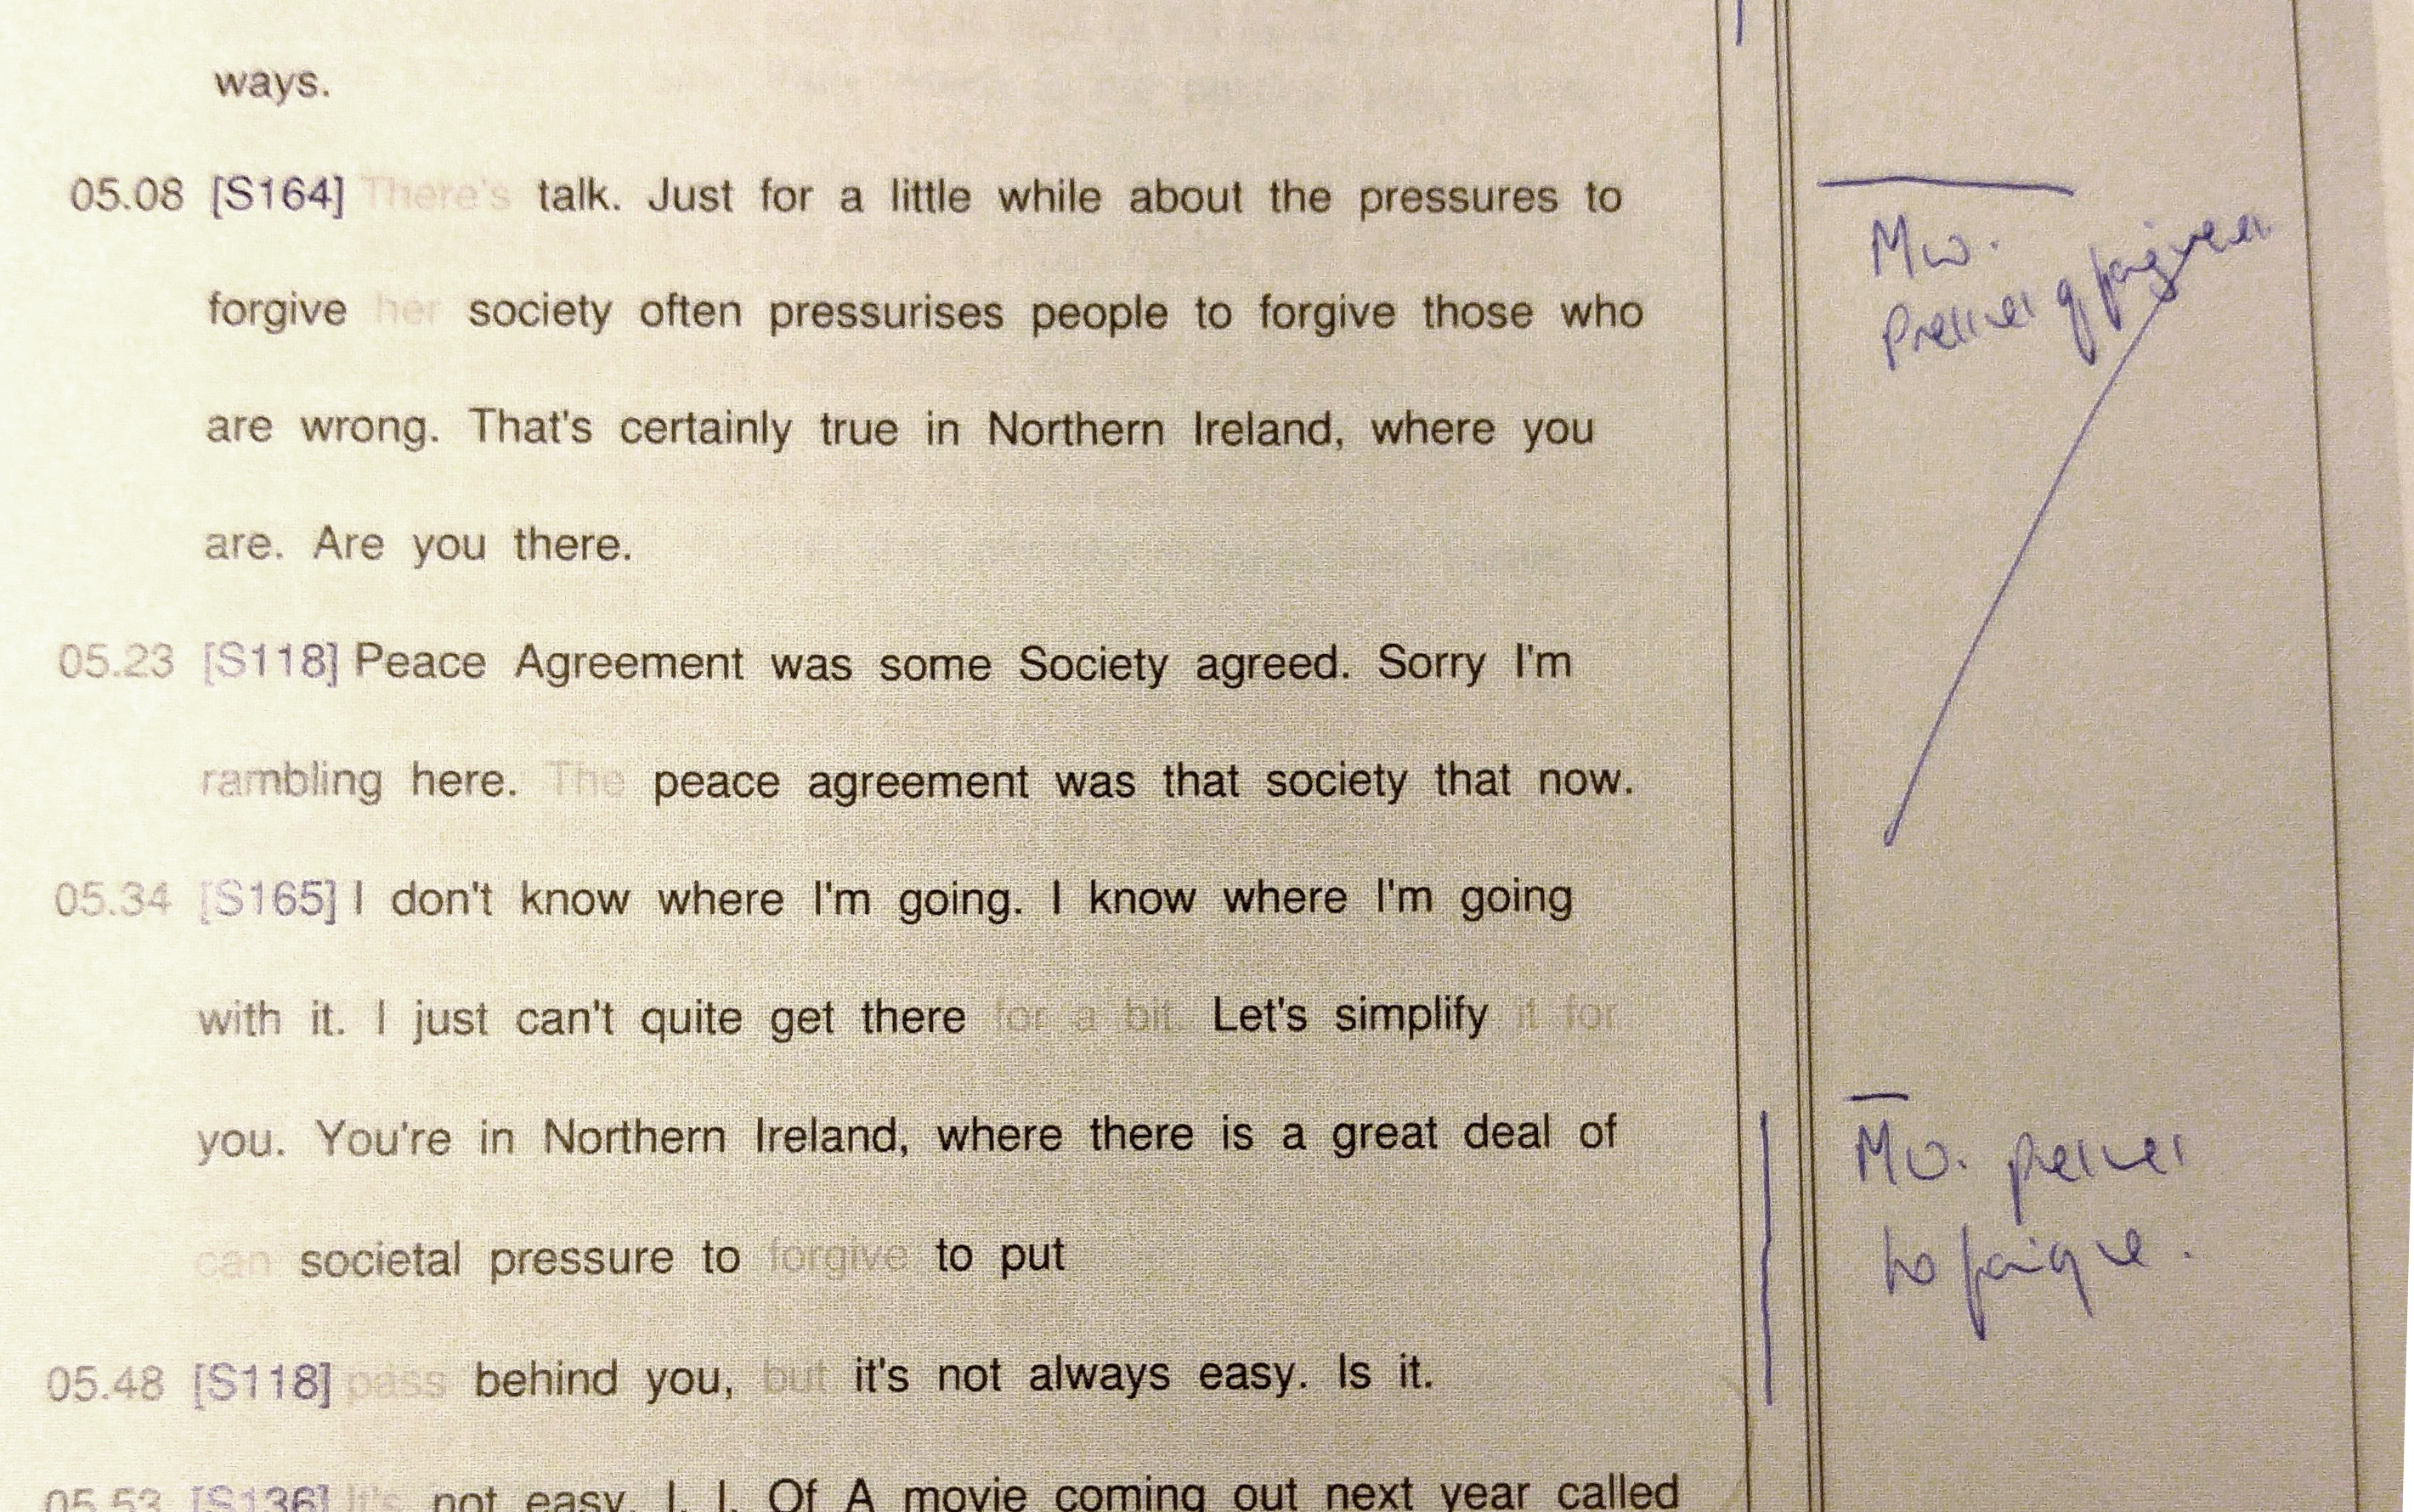
\includegraphics[width=\columnwidth]{figs/pen-annotations-p5-cropped.jpg}
  %\caption{Annotations made by P5. The content is segmented using horizontal lines and labels in the margin. The
  %middle segment is marked as not needed using a diagonal line.}
  %\label{fig:p5-annotations}
%\end{figure}

By capturing this information in a structured way, it could be exported as part of the EDL to guide the producer in
later stages.  P3 suggested that it might be possible to automatically generate labels using the text of a selected
clip.

\textit{``If it was to dump those separate clips in your [system] and name them according to the text, then that would
save twenty minutes suddenly in a single go.''} (P3)

% For instance, I'm doing the transcript was about Guantanamo and one was like okay there are three categories of
% prisoners and at one point I was quite tempted to be able to like label this. The whole thing. o.k. All audio
% could work for the forever prisoners and that other bit of audio... and that's in a way what you would do with SADiE
% or StarTrack You could kind of name your clips (P6)

\subsubsection{Annotation}

%TODO P6 created a Box document to take notes

% HIGHLIGHTER PEN

%Participants used a variety of annotations as part of their editing workflow. Most used some form of highlighting to
%select the parts they judged to be particularly good.

PaperClip used an underlining gesture to select words, but P1 and P6 both suggested that they would prefer using a
highlighter pen style mark.  This would also mean that the transcript wouldn't have to be double-spaced, but it would
require a system that can distinguish between a strikethrough and highlight.

%\textit{``You did an underline, but I would like to have it as a highlighter pen as you've got that option on Word''}
%(P1)

Participants used different marks to rate the importance of their selections, including stars and asterisks, which we
witnessed previously in Chapter~\ref{chp:screen}. However, both P2 and P6 suggested using colours as a way of marking
up different selections.  This could be used as a rating system, where one colour is considered more important than
other, or as a categorical system for whatever context is appropriate to that producer.

\textit{``Maybe if you had different colours you could mark your first one in red [then]
  %and this was like kind of o.k. The first draft and you say okay, that I like. And then you'd go through it and somehow could
change colour and underline it a second time.''} (P6)

%\textit{``I was just labelling by summarising a paragraph in about two or three words --- just who is speaking and the
%substance of it --- or maybe just putting a cue to say that was a question.''} (P5) 

%P7 said they were interested in including additional metadata like music reporting data. This is required when music is
%included in a programme, so capturing this data in a structured way would save them having to complete and submit a
%music reporting form.

%\textit{``What I've started doing as a PasB information is adding in music details for post-production''} (P7)

% COLOURS

\subsubsection{Interface}

%All of the systems we tested used the same transcription system, but presented the transcript to the participants
%through different interfaces. When participants compared the systems, we did not find that there was any clear
%`winner', but that the interfaces had strengths in different areas. The feedback we received from participants
%indicated that the fuller functionality of the screen may make it better for more intensive editing, where producers
%may not be sure what they want from a recording, while the more lightweight pen system may be better for quickly
%selecting and removing content, when it is already known what is needed.

%One of the frustrations expressed by participants about their current workflow was that they have to use multiple
%different systems to put their programmes together. Often these systems have poor or zero integration, and the
%interfaces have variations such as different keyboard shortcuts for the same task.

%\textit{``We're darting in and out of five different systems a day, so we're editing in ProTools or writing emails or
%doing this, and they've all got slight differentiations''} (P7)
%%so sometimes you go 'oh, f*** it - I can't remember what it is I needed to do on that.

%P3 and P6 said they enjoyed that the screen interface had all of the features available in the same place. The playback
%of the audio was integrated into the interface, and they could correct and annotate the text, then export it without
%having to use separate systems for audio playback or word processing. The pen interface did not support integrated
%playback or correction while in use.

The lack of integrated audio playback and navigation in the pen interface made it more difficult for participants to
navigate the audio content.  Although participants could use a separate playback device to navigate the audio,
they either had to do this ``blind'', or use the timestamps on the transcript to guide themselves to the desired
position. With the screen interface, participants could use the text to see where they were navigating to, making it
much easier to move around non-linearly.  We observed that when using the pen interface, many participants chose to
edit while listening straight-through, without navigating the audio at all.

The ease of navigation offered by the screen interface may make it better suited to editing recordings where producers
are more reliant on listening to the audio. This could include content with which the producer is less familiar, such
as a recording they were not present at, or a recording from the archive.

\textit{``I think if you're in a rush, and you know roughly what you've got, and it's an interview that's close to
memory, then the pen's really good. I think if you want to get into the guts of the interview, [...] then you're going
to want to work on the screen.''} (P7)

\subsubsection{Export}

Both the screen and pen interfaces that we tested included a feature to export an edit decision list (EDL) to a DAW.
This allowed the participants to integrate with their existing workflow by being able to make changes to their edits
using their existing tools.  P2 and P6 expressed frustration that annotations were not included in the export.

\textit{``Once you have put it into SADiE you have to [label the content] again. It's almost like you've gone forwards
then you have to take half a step back and you lose a bit of momentum.''} (P2)

%If user annotations could be captured in a structured way, then they could be used to label the clips 
%in the EDL.

The other frustration with the export feature was that in the EDL, the selected clips were all pushed together without
any gaps. P3, P5 and P6 said that they would like there to have been gaps between clips, so that it would be more
obvious where the edits are when listening back. Instead of using gaps P5 and P8 moved their selected clips to a
different track in the DAW when editing with the normal printed transcripts. This also allowed them to see where the
clips were located in the original recording.

%\begin{figure}[h]
  %\centering
  %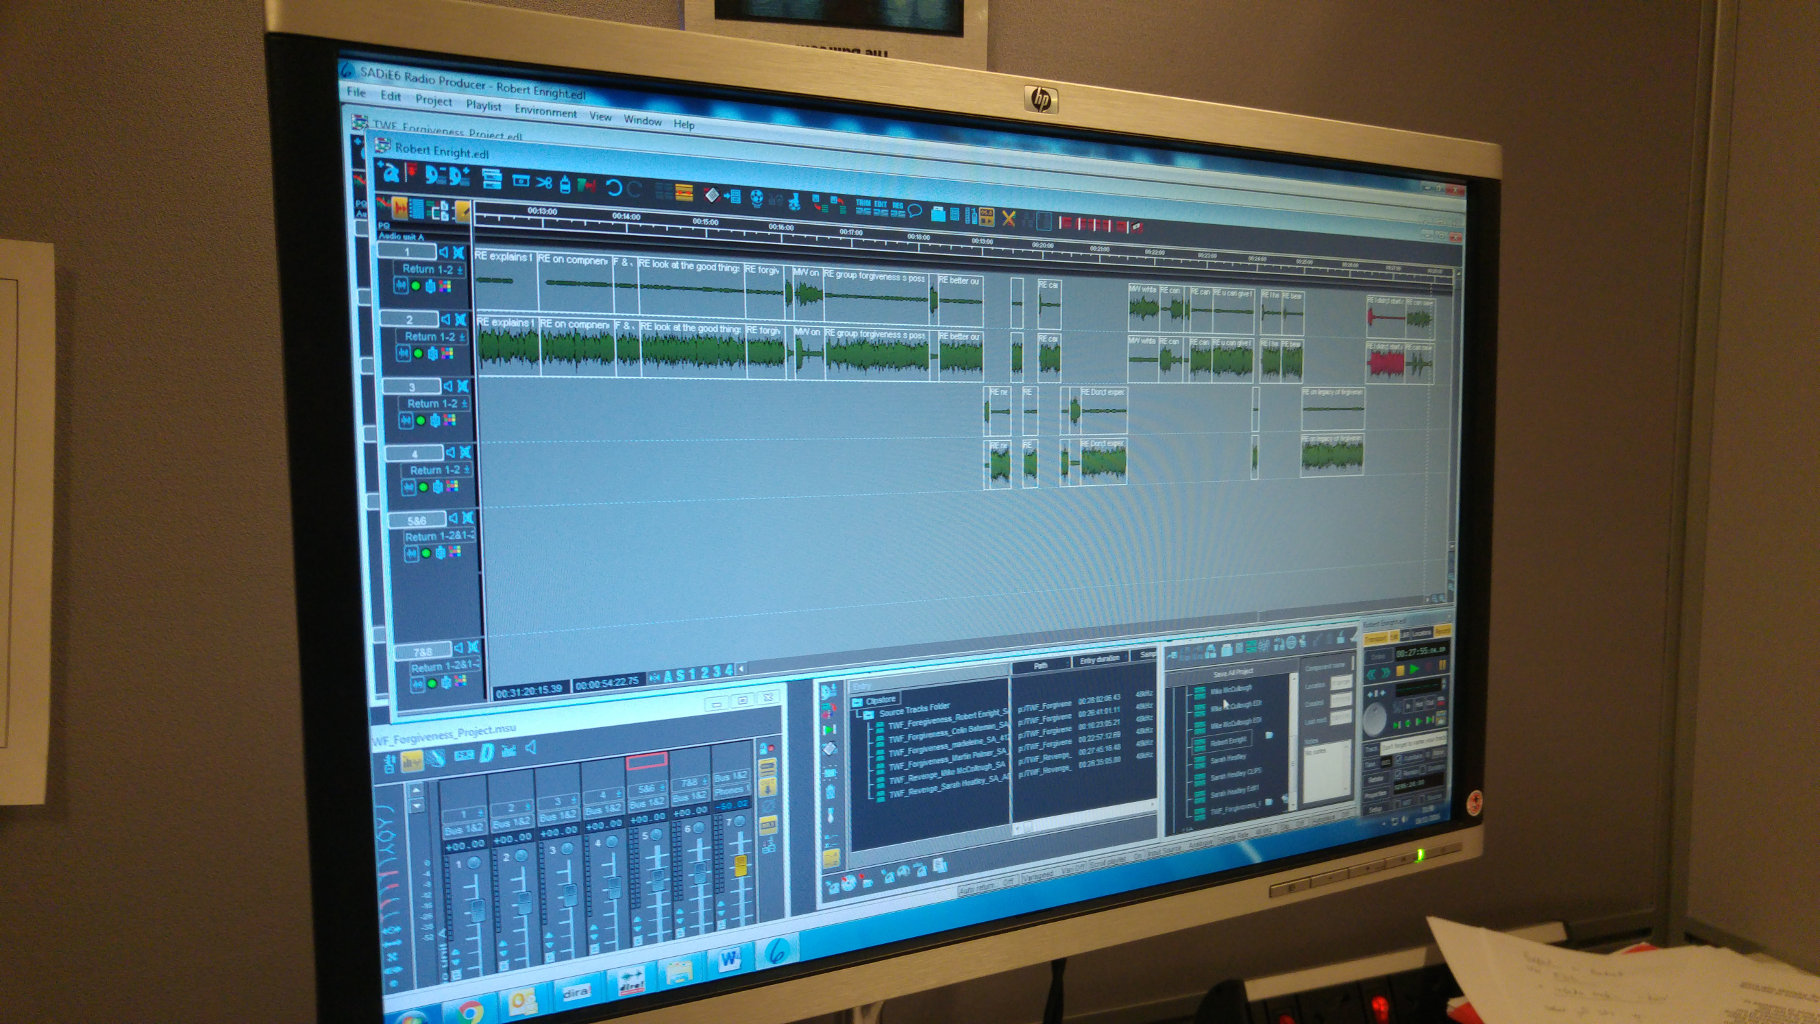
\includegraphics[width=\columnwidth]{figs/pen-screen-p5-lowres.jpg}
  %\caption{P5 moved their selected clips to a separate track}
  %\label{fig:p5-screen}
%\end{figure}

\subsection{Transcript}

% ======================== PAPER
\subsubsection{Paper}

Most participants commented that working with paper had a number of benefits to their workflow.  P2, P5 and P8 said
they found it easier to read from paper than screen.  P1, P2, P6 and P7 said that it was easier on the eye and gave
them a break from working on screen.  P2, P5 and P7 said they enjoyed that paper was a physical, tangible medium which
they could touch.  P1 and P5 commented that using paper transcripts made it easier for them to orientate themselves.


P1 said the paper interface allowed them to think more widely, and P8 reported that they found it easier to remember
the content of the transcript when reading on paper rather than a screen. 

%\textit{``I find it easier to read on on paper.''} (P2)

%\textit{``I much prefer to have paper. Even if I've got them on screen, [...]
%%. Um. I do use them on screen, but I.
%I do find the paper version easier.''} (P5)

%\textit{``If I've got a lengthy article, I won't even... well, I'll start off reading it on screen to check whether or
%not it's relevant, but then I'll just have to stop and print it.''} (P5)

\textit{``I find it easier to read off paper, and easier to remember stuff.''} (P8)

\textit{``It's essential to print [because]
  %%. I think I especially if you're doing the first thing with the SADiE
  %%I like to have the transcripts printed out because at the moment how I work is
  %I have the transcripts on my computer, but I still need to print them out to be able to edit because when I'm
  %coming to write this script,
I have to think more widely. What bits am I going to put where? What's my
  structure? Where am I going to put this bit? Mentally, it is easier for me to refer to the [paper] transcript so
that I know where everything is.''} (P1)
%%for when it comes to me actually using one of the bits. that I want

%\textit{``I think I just prefer to have a printed version. I find it kind of easier to have that to hand all the time,
%rather than having to flick through screens all the time, back and forth through screens.''} (P1)

%\textit{``On the screen it's always the same quality, but [with] a fingered piece of paper [...]
  %%can be a bit comforting as well.
%you think, `this is not new to me', even if it feels new, I've been over this before.''} (P5)

% =============== ACCURACY
\subsubsection{Accuracy}

All of the participants were successfully able to use the ASR transcripts to edit their material as
part of the production of their radio programme, and all reported that the transcripts were sufficiently accurate for
the purpose of editing their content. Similarly to what we found in Chapter~\ref{chp:screen}, the most common
complaints were of reduced accuracy due to heavy accents or background noise, and problems with speaker labelling and
confidence shading. For example, the ASR system would occasionally give a high confidence score to an
incorrect word, or a low confidence score to a correct word, which caused P3 to mistrust the confidence shading.

\textit{``The things it wasn't sure about weren't actually very often the real mistakes.''} (P3)

%The speech-to-text system also included a post-processing stage which punctuated the transcript. This was expected to
%make the transcript easier to read, but P4 reported that they found the errors in the punctuation distracting and were
%interested in correcting those mistakes. However, this was not mentioned by other participants.

% CONSEQUENCES

P6 normally works with perfect transcripts and found that the errors by the ASR system caused them to rely more on
the audio than they normally would, although P7 and P8 said they could use their memory to ignore many of the mistakes
in the transcript.  P8 reported that lower accuracy transcripts caused them to make rougher edits than they would
normally.

%\textit{``Obviously reading back, it'll slow you down if it's completely the wrong word.''} (P2)

%\textit{``I'm used to working with a transcript that is 100\% accurate, which means I don't have to go back to the
  %audio as much. With [these systems], I had to go back to the audio more than I was used to, so I did feel that slowed
%me down a little bit.''} (P6)

%\textit{``The English was a bit confusing so I felt on that one, I could only do quite gross editing, topping and
%tailing and taking chunks out.''} (P8)

%\textit{``The fact that it wasn't very accurate in places made it difficult [partly because] it's been a long time
%since I did those interviews. Normally it wouldn't be such a big break between recording and editing them.''} (P8)

% =============== CORRECTION
\subsubsection{Correction}

We observed that all of the participants chose only to correct errors that impacted on their ability to
read the transcript.  P2, P4 and P6 said that gross inaccuracies in the transcript distracted them, which caused them
to read more slowly and reduced their editing speed.

\textit{``It's good to have the option to sharpen it up as you go along because, obviously, reading back it'll slow
you down if it's completely the wrong word.''} (P2)

% REPEAT ERRORS

We observed that the ASR system would often make repeated mistakes on an unknown word by mistranscribing it
as a variety of words, which made it difficult to fix.  This usually occurred with names of contributors, or words
specific to the topic of the programme.  P3 and P7 asked whether it would be possible to provide custom training to the
ASR system to tailor it for their specific programme.

\textit{``If you're doing a story about AIDS, there's going to be stuff about anti-retrovirals [...]
  %or something like that
  %and even in  quite mainstream subjects there is going to be some special vocabulary. Anyway, I just think that you
  %could. I'm just wondering. I can see that it would be a bit of extra trouble. But it seems like it's something that
The ability to teach it some words would be really good.''} (P3)


% ================ GENERATION
\subsubsection{Generation}

The participants in this study re-iterated the finding from Chapter~\ref{chp:screen} regarding frustrations with manual
transcription and the benefits of having the transcript automatically generated.
P1 and P3 stated that the ASR element was the largest benefit of the semantic speech editing systems, as it
freed up that time.

\textit{``The transcription thing for me is eighty percent of the advantage.''} (P3)

P7 reported that they already make regular use of a commercial ASR system called
\textit{VoiceBase}\footnote{\url{https://www.voicebase.com/}, accessed 18/01/2018.} to automatically generate
transcripts.  P5 had previously tried a different commercial system called
\textit{Trint}\footnote{\url{https://trint.com/}, accessed 18/01/2018}, but could not continue due to the cost. None of
the other participants reported having used automatic transcripts as part of their existing workflows.

%P1 worked on programmes for the BBC World Service, which covers current affair stories around the world.  They often
%have to deal with recordings of speech in foreign languages, which is especially tricky when they don't speak the
%language.  The recordings and translation are then normally sent to a colleague who can record translated speech of the
%parts the producer is interested in using. These are then dubbed over the original recording. However, it can be
%difficult to know where to position the translation over the original, as there are no timing references provided.  P1
%said that their department spends money on translation services to help with this process.

%\textit{``This department doesn't realise how much money they spend on [...] translation. I don't know if you can do
%[semantic editing] in a different language?''} (P1)

%Our ASR transcripts could be processed with automated translation to enable producers to navigate audio content
%in their native language. There may also be scope to provide some level of editing capability, but due to differences
%in word ordering (e.g. adjectives before/after nouns), the editing may only be possible at the sentence level. However,
%the success of this is dependent on the accuracy of the translation, and P1 suggested this may require a good human
%translator.

%\textit{``I've had bad translators and just [received] gobbledygook as they've done a literal translation. I mean
%Google Translate doesn't make any sense at all.''} (P1)

\subsection{Listening}

% ======================= CRITERIA
\subsubsection{Criteria}

All of the participants chose to listen to the audio while editing with the transcripts. They gave four reasons for
doing so: processing information, efficient navigation, judging quality and identifying non-speech sounds.

P1, P4 and P6 reported that listening while editing made it easier for them to process the information that was being
communicated in the interviews.  P1 and P6 said this helped them to find where corrections needed to be made and to find
words that were inaudible or not actually present.  P2 and P8 suggested that the multi-modal input of listening and
reading helped them to understand the content and make edit decisions.

\textit{``I think reading and listening at the same time makes it easier to take that amount of information on. It's
going into two sensory inputs so it's easier.''} (P8)

%\textit{``It sort of reinforces what you're reading and vice versa.''} (P2)


%\textit{``I would like to hear the clips that I've underlined to know [...] how it sounds as a standalone clip, because
%with some bits I started somewhere and ended somewhere else, so I wanna put them together.''} (P1)

%\textit{``I need to be able to [listen] at the same time because if I'm just doing it on the paper with the pen, I
%can't hear what they're saying. Most of the time it's not really the words, it's how they're saying it.''} (P1)

Although a transcript can tell you what was said, it does not tell you how it was said. This can change the meaning of
the words, and make the difference between an edit that works or not.
One thing the participants were looking out for were any low quality sounds such as ``umm''s and breaths, which are
distracting to listeners and can reduce the intelligibility of the speech.
The ASR process does not attempt to
transcribe ``umm''s, breaths or non-speech sounds. This means that producers must listen to identify these.
P7 and P8 showed an interest in using the transcript to remove these noises.

%and non-speech sounds like environmental
%sounds and music, which are used to enrich the listening experience.

P1 was interested in hearing the direction of intonation, that is, whether the voice rises or falls in pitch.
The intonation at the end of a clip must match the beginning of the next clip, otherwise it will be
apparent to the listener that the two have been cut from different parts of a recording. Such information is not
visible using the transcript.

\textit{``It could be that [...] the intonation is going up and it won't work as a clip, so I need to hear it.''} (P1)


%\textit{``[The edit] might look all right there, and I know this is generally what they're saying here, but [...]
%%when it comes to actually getting that clip, I want to hear the clip So it's all right for a really rough. just
%%an idea. at a really early stage. But for me
%once you get onto an editing stage, even if it's a rough edit, I need to be able to hear it.''} (P1)


%\textit{``If I was making a heavily actuality-led programme, I wouldn't bother with those sort of transcripts, because
%what you want is the sense of the sound, of its audio environment.''} (P7)

%\textit{``It would have been interesting to have done this with a project where you need to be listening for very
  %different things. [I wonder] whether one could mark up on the transcript `atmosphere change here', `big rain cloud
%there', `thunderstorm here', because you need to know where they are.''} (P7)



% ===========================TECHNIQUE
\subsubsection{Technique}

P4, P6, P7 and P8 all said that they sometimes edit using only the audio itself. When the audio recording 
is short enough that the producer can remember what was said and where, then there is less need for a transcript. P4
put the cut-off threshold as 15--25 minutes.

  %[Transcripts are] good to have a if you've got a long interview. I think 
\textit{``For interviews that are under 15 minutes, I can hold the whole thing in my head. [...] For things
that are over 25 minutes, then that's when [transcripts] start to become useful.''} (P4)

Some programmes focus more on the auditory experience than the words by combining field recordings, sound effects and
music.  In these cases, there may be little benefit in using transcripts at all.

\textit{``If I was making a heavily `actuality-led' programme, I wouldn't bother with those sort of transcripts because
what you want is the sense of the sound, of its audio environment.''} (P7)

P1 and P7 reported that their existing editing workflow often involves re-listening to the material they recorded in
full, \textit{``from beginning to end''} (P1). They reported that this allows them to refresh their memory, and to
start making decisions on what to lose or to keep.
%\textit{``I would go through every single interview and listen through it, from beginning to end.''} (P1)
P2 said that they found manual transcription to be a good opportunity to re-listen to material for similar
reasons.
%\textit{``Logging is good in some ways in terms of the process --- you sit, you listen back, you write it down, you
%underline your key bits --- but it's also a clerical thing that takes a lot of time, which we don't really have.''} (P2)
Although removing the requirement to manually transcribe recordings reduces the burden on producers, there is a risk
that it takes away an opportunity to re-listen to material. This may introduce an unintended negative impact in that
edit decisions are based more on the words that are spoken and less on how the programme sounds.

% ============================= NAVIGATION
\subsubsection{Navigation}

%\textit{``I had to go back several times to see if I could match something from the end of his answer to the beginning [...]
  %That kind of jumping around wouldn't be possible [...]
  %%with I mean it would be possible
%with the pen because of the way I was listening.''} (P4)

%\textit{``If it got a bit waffly then I'd start looking at the transcription and [...]
  %%think `okay how much longer is this going to go on?', um o.k. It goes on for another two minutes so Right, well I'll
%just skip ahead to the next question.''} (P4) 

P2, P4, P5 and P7 spoke of how they used listening in combination with the transcript to efficiently navigate and edit
the audio. They did this by skipping forwards when what they were hearing was not usable, jumping backwards to review
content that had already been listened to, and seeing if the upcoming audio was something of interest.  If it was not,
then they could avoid listening to it altogether, which would save them time.

\textit{``You can glance at the transcript and just see there's a paragraph of stuff that really is not really relevant
  %. Even though it's quite interesting. So you can glance down. See that summarise it's about a giraffe and you want
  %stuff on A rhino
[...] and just discount it, whereas with your ears you've got to listen to the whole thing.''} (P5) 

As we saw in Chapter~\ref{chp:screen}, most participants increased the playback speed when listening using the screen
interface or their DAW to skip through material they thought they might not want to use.

%\textit{``If you know it's going to be a boring bit, you can just go fast.''} (P8)



\section{Discussion}\label{sec:paper-discussion}

Through our evaluation study, we achieved our aim of understanding how the radio production workflow was affected by
our paper interface, compared to a screen interface. We also gained further insights into how the accuracy of ASR
transcripts affect the editing process, and how listening is used to complement or replace semantic editing.
We discuss each of these topics below.

%In this chapter, we were interested in exploring the relative benefits of semantic editing of speech using a pen-based 
%interface, compared to a screen-based interface.
%We found that the behaviour of participants was different between the pen and screen. With the pen interface,
%participants make quick decisions on selecting or removing content, while with the screen, they corrected some words
%and navigated the audio to make more considered decisions. The screen interface allowed participant to correct the
%transcript while they edited, giving them a richer output, while the pen did not.


%There was no integration between the pen interface and audio playback. Although this did not prevent the participants
%from navigating the audio, many did not do so, which meant that they edited the audio straight through in real-time. 
%The pen interface also did not include any functionality for correcting mistakes in the transcript. Although this meant
%that the mistakes were still present after editing, the participants were not distracted by making corrections, so they
%could get on with making edit decisions.

%In their interviews, participants talked about the benefits of using paper. It is already known that reading from paper
%rather than from a screen allows readers to gain a deeper understanding, cross-reference and interleave reading and
%writing.  The comments made by participants suggest that these finding also seem to apply to semantic speech editing on
%paper. Additionally, there were some suggestions that it may be easier to listen and annotate simultaneously, and
%easier to make edit decisions when using paper.

%There are a number of improvements that could be make to the pen interface, which may have caused it to be rated as
%less usable and useful than the other systems we tested. One of the main benefits of working on
%paper is that it can be annotated freely. However, the system we used to build our prototype forced users to draw only
%within a margin, and to edit by drawing strictly within defined borders. This caused many participants to be concerned
%about introducing errors by drawing outside of the lines, and did also not like not being able to draw freely.
%Future systems should consider using a more advanced system that takes a less literal approach to annotations.

%The screen interface added two features over the pen interface --- integrated playback and correction. The ability to
%navigate the audio playback using the transcript allowed the participants to skip forwards and backwards easily
%without having to use timestamps. This lowered the barrier to replaying content that was of interest, or reading ahead
%in the transcript and skipping over content that was not of interest.

%In the screen interface, the transcript could be corrected while editing. With the pen interface, correction was not
%possible on paper, but could be done using the screen interface before printing it out.


%PEN
% most popular, fastest, but rated least usable and useful
% simplicity and lack of navigation/correction may have led to increased speed
% lack of integration with listening may have led participants to use interface differently from screen
% participants talked about benefits of using paper - easier to read, remember, make decisions, orientation
% did not include correction or detect written notes
% strictness of gesture detection has potential to introduce errors

% SCREEN
% included correction, participants mised correction with editing
% distraction of correction may have slowed edit time
% ease of navigation makes it more suitable for exploring content, experimenting

% NORMAL
% Quarter of participants didn't want to continue using semantic editor
% Familiarity, reliability are important when workflows are tight

\subsection{Paper vs screen}

%Editing is a multi-stage process. Participants said that the interfaces we tested were best suited to the first rough
%editing stage. This may be due to lack of features for organising and re-ordering content. We addressed this by
%integrating with DAWs, but the transcripts are lost through this process. Adding features for labelling and re-ordering
%would allow users to use transcripts for the later stages of editing.

We found that there were no overall preferences between the paper and screen interfaces, but that there were
advantages and disadvantages of both in different uses and circumstances. Influential factors included the complexity
of the edit, familiarity with the audio, accuracy of the transcript, user location and collaboration.  Broadly speaking,
we found that our pen interface was better for making simple edits involving quick decisions, using familiar content
with a high-quality transcript, for producers working away from their desk, or with others in the same room.  By
contrast, we found that our screen interface was better suited to more complicated editing involving complex decisions,
using less familiar content with a lower accuracy transcript, for producers working at their desk, or with other people
remotely.

% other
Participants reported that using paper rather than a screen made it it easier to read transcripts, remember
information, think widely and orientate themselves. This aligns with previous research that has compared reading on
paper to screens \citep{OHara1997,Kurniawan2001,Mangen2013,Singer2017}. These results show that the benefits of
paper-based working can translate to radio production using ASR transcripts.

On average, editing using the pen interface was 16\% faster than using the screen, but this result was not
statistically significant.
However, three of the participants reported that they could edit faster and more easily using the pen interface compared to the
screen.
%Additionally, the mean relative edit time of the pen was faster than the screen, but this was not statistically
%significant.
This may have been partially due to the faster reading speed of paper and the ability to underline while reading or
listening.  Some participants also suggested that the lack of integrated playback and correction features may have
caused them to focus more on the task at hand, rather than being distracted by correction or navigation.

% integrated playback and correction
The screen interface included integrated playback and correction, which made it a more powerful tool.  P7 reported that
this made it suitable for more challenging editing tasks or exploring less familiar content, where the producer needs
to be able to listen and navigate efficiently. The integrated listening also made it better for working with less
familiar or lower accuracy transcripts as participants could tolerate the errors by using their memory of what was
said, by listening or by correcting the errors. The screen makes it easier to listen and correct the errors, so is a
better choice for editing less familiar content or lower quality transcript. 


% improvements
Three participants reported that both interfaces lacked features for labelling or re-ordering material, which meant
that they were only currently suitable for creating a rough edit. This limits the usefulness of semantic editing in the
later stages of production. For the pen interface, handwriting recognition could be used to label a specified region,
or the nearest selected content. Two participants requested that the labels should be included in the exported EDL, so
that they integrate with their existing tools.
%Two other participants said they would prefer to use a highlighter pen than to underline, and others suggested using
%multiple ink colours to label content or to indicate multiple iterations.  However, we are not aware of any digital
%pens that support highlighting or quickly swapping nibs.

% portability
Half of the participants reported that they like to work away from their desk or office as it helps them to focus. Pen
and paper is naturally very portable and can be used almost anywhere. As it is does not use a screen, it is smaller,
lighter, easier on the eyes and has a longer battery life. Several participants reported that this makes it more
suitable for travel, and would allow them to work in more comfortable places. However, the requirement to print the
transcripts makes it unsuitable for working ``on the road'', where new material is recorded outside the office. By
using a laptop or tablet device, the screen interface is also portable. The screen has the advantage of
integrated playback and correction, and could be used on the road as it doesn't need a printer.

% collaboration
Producers do not work alone and need to collaborate with others during production. The physical nature of paper made
the digital pen interface suitable for working with others in the same room, as it allowed them to spatially arrange
the pages and refer to the transcript by pointing. However, it is not possible for the pen interface to be used
remotely. The digital nature of the screen interface makes it easy to work with remote collaborators. There is also
potential to extend the screen interface to use operational transformation \citep{Sun2004}, which would allow multiple
users to edit the same content simultaneously.

% implementation constraints
Our choice of technology for implementing the pen interface introduced some constraints that affected our design.
Users edited the content by underlining or striking text within a set of rectangular boxes. These gestures were
interpreted literally, which created a potential source of errors, and forced the participants to draw carefully. This
design also prevented us from including correction and undo features. The batch-mode operation of the digital pen also
prevented us from including integrated playback.  By overcoming the constraints of our implementation, a pen interface
with integrated listening, correction and undo could allow users to combine the benefits of working with paper with the
full feature-set of the screen interface. However, there is also a risk that adding more features to the pen
interface could introduce distractions, as we saw with the screen interface.
%TODO Mention undo approach in Olberding2010

Electronic paper may provide a technical solution that could bypass these constraints. At the time we developed our pen
interface, there were no e-paper devices that supported digital ink interaction, but these will become available in the
near future.  For example, the \textit{reMarkable} tablet\footnote{\url{https://remarkable.com/}} is an e-paper device
that includes a digital ink interface. Although e-paper displays do not seem to currently perform as well as paper for
reading speed, comprehension or eye fatigue \citep{Jeong2012, Daniel2013}, they are likely to improve over time and may
provide a good middle-ground between paper and screen interfaces. 


%As humans are not
%good at drawing straight lines in freehand, it would be better to create a system that was more forgiving in this
%respect.

%The quantatative data we collected did not produce any statistically significant results and produced very mixed
%messages. On the one hand, half of the participants selected the pen interface as the system they would prefer to
%continue using, and it had the fastest mean relative edit time. However, the participants also rated the pen interface
%as the least usable and least useful of the three.  Despite it having no semantic editing capability, the participants
%rated the normal paper interface as most usable and useful, and a quarter selected it as the preferred option.
%Based on this data, it is not possible to draw any conclusions.

\subsection{ASR transcripts}


%All of the participants were able to use the automated transcript to edit speech recordings for their radio programme,
%supporting what we found in Chapter~\ref{chp:screen}. One of the participants in this study had already started using
%ASR as part of their normal workflow. As automated transcription becomes more widely available, it is
%important to design tools that make the best use of the extra information.

%As the semantic editing tools we tested are based around transcripts, 
The accuracy of a transcript has a direct effect on the performance and usage of semantic editing tools. We identified
five different areas that were affected by transcript accuracy: correction, reading speed, reliance on listening,
transcript longevity and edit granularity.

Three participants reported that errors in the transcripts slowed down their reading speed, with some errors being more
distracting than others.  Clearly, the more errors that occur, the more likely it is that corrections will be needed.
However, the majority of participants were only interested in correcting errors that were particularly distracting.
None of the participants needed or wanted to fully correct the transcripts, as this is only required if the transcript
needs to be published. Although publication of transcripts is not currently part of the production
workflow, doing so would make the programmes more easily discoverable and searchable.

The ASR system we used often mistranscribed unknown words into a variety of different words, which prevented the use of
search-and-replace.  This usually occurred with words specific to the programme, such as names of contributors or
locations. To avoid this, producers could add unknown words to the dictionary of the ASR system prior to transcription.
By providing additional contextual information, such as the programme topic or number of speakers, the ASR system could
improve the transcript accuracy by using this to better calculate the likelihood of certain words occurring or by
limiting the number of unique speaker segments.

%% listening/memory, longevity
The participants in our study using listening and memory to tolerate errors in the transcript.  Remembering what was
originally said increased the readability of the transcript and reduced the need to replay the audio.  One participant
reported that transcripts are often retained to help producers search through previously recorded material. However, as
the producer's memory fades, the errors in the transcript of previously recorded material become more of a problem, and
the usefulness of the transcript deteriorates over time.

% edit granularity
One participant reported that they selected more material than they needed due to the number of errors in the
transcript.  This suggests that the accuracy of the transcript may affect edit granularity.  Selecting too much
material creates more work for the producer at a later stage, as they have to edit their programme down to a
specific time.

Two participants showed an interest in using semantic editing to remove ``umm''s and breaths. The ASR systems we used
were designed to ignore these sort of noises, rather than transcribe them. When they did appear, they were transcribed
into a variety of words, which made it difficult to find and remove them. By explicitly including ``umm''s and breaths
in the ASR training data, these noises could be highlighted in the transcript, which could give users the option to
remove them automatically.

%% suggestions
%One participant suggested that semantic editing could be used to handle speech content in a different language.
%Timestamp information is necessary for semantic editing, and by using an automated transcription process, we could map
%the original timestamps of the transcript to the translated text.  However, the different grammatical rules of
%different languages mean this mapping would be complex, and may limit the granularity of editing to whole sentences
%rather than individual words.  Also, in the experience of the producer in question, the quality of automated
%translation is not yet high enough to replace human translation. 

\subsection{Listening}

We found in Chapter~\ref{chp:screen} that listening was an important part of the editing process. Through our study, we
learned more about how and why the participants listened to the audio for semantic speech editing.  Participants gave
three main reasons for listening --- processing information, judging sound quality and identifying non-speech sounds.

Listening allowed participants to hear what the transcript could not tell them, such as identifying mistakes or
omissions in the transcript, finding where there are environmental sounds and working out whether the quality of the
speech is sufficiently good for inclusion in their programme.  Two participants said that simultaneously reading and
listening made it easier to process the information in the speech, making the edit process more efficient. This falls
in line with previous findings that providing transcripts allows users to process voicemail messages more efficiently
\citep{Whittaker2002}, and improves the comprehension of time-compressed audio \citep{Vemuri2004}.

% no need for transcripts
Half of the participants reported that they sometimes edit audio without a transcript, as they can remember most of
what was said, and when it was said, for audio recordings less than 15--25 minutes long.  For some programmes that
focus on the auditory experience, editorial decisions will be led by the quality of the sound rather than what was
said. In these cases, the cost and overhead of generating a transcript may not be worthwhile, however, it is unclear
exactly where this threshold lies.

% re-listening
Two participants reported that they like to re-listen to their recordings in full to refresh their memory and start
making decisions on what to use for their programme.  Another participant suggested that the current process of manual
transcription gave them an opportunity to re-listen.  Re-listening in full adds overhead to the editing process, but
some participants considered it to be a worthwhile process.  The introduction of ASR transcription removes this
opportunity. There is a risk that semantic editing may cause producers to base their decisions on transcripts rather
than audio, which may affect the quality of the programme.

% improvements
Listening is an important part of editing, but it is a time-consuming process. This could be reduced by using time
compression techniques to increase the playback speed, as discussed in Section~\ref{sec:background-time-compression},
or using sound event detection to identify and label regions of environmental noise \citep{Duan2014,Kroos2017}.
Including this information in the transcript could help producers identify sounds they do or do not want.  Producers
may also benefit from tools that help them see which edits would work or not.  For example, a graphical representation
of the intonation of speech may help producers identify whether editing two pieces of speech together would sound
acceptable.

\section{Conclusion}\label{sec:paper-conclusion}
We presented the results of a contextual user study of semantic speech editing in professional radio production that
compared a digital pen interface to a screen-based interface.  We found that the pen and screen interfaces both work
well, but that each is better in different situations.

The benefits of reading from paper and the simplicity of the pen interface made it better for fast, simple editing with
familiar audio and accurate transcripts.  The integrated listening and correction features of the screen interface made
it better for more complex editing with less familiar audio and less accurate transcripts.  Unlike the pen, the screen
interface is capable of remote collaboration, but the pen interface may work better when working with others
face-to-face.  The digital pen provides greater flexibility for working away from the desk, but its dependence on
printing makes it difficult to work on the road.  The lack of re-ordering and labelling features in both systems
prevented them from being used beyond rough edit stage.

The accuracy of transcripts is crucial to success of both systems. Lower accuracy transcripts appear to result in more
correction, slower reading speed, more reliance on listening, a shorter transcript ``shelf-life'' and selecting more
audio than necessary. The accuracy could be improved by using programme-specific information in the ASR process.
Listening is an important part of the editing process, with some producers choosing to re-listen to recordings in full.
Listening is used to process information, judge quality and identify non-speech sounds. Transcripts may not be needed
for short recordings or where the auditory experience, rather than the specific speech content, is particularly
important.

